\documentclass[11pt,letterpaper,notitlepage]{article}
\usepackage[left=1in,right=1in,top=1in,bottom=1in]{geometry}
\usepackage[dvipsnames]{xcolor}
\definecolor{darkblue}{RGB}{46,48,147}
\usepackage{hyperref}
\hypersetup{colorlinks=true,
            linkcolor=darkblue,
            urlcolor=darkblue,
            citecolor=darkblue}
\usepackage{xspace}
\usepackage{amsmath,amsfonts,amssymb}
\usepackage{lipsum}
\usepackage[utf8]{inputenc}
\usepackage[T1]{fontenc}
\usepackage{palatino}
\usepackage{mathpazo}
\usepackage{ifthen}
\newboolean{cms@italic}
\setboolean{cms@italic}{false}
\newboolean{cms@external}
\setboolean{cms@external}{false}
\usepackage[pazoGreek]{heppennames2}
\usepackage{ptdr-definitions}
\usepackage{lastpage}
\usepackage{fancyhdr}
\usepackage{graphicx}
\renewcommand{\headrulewidth}{0pt}
\lhead{Javier M. Duarte}
\rhead{Personal Statement}
\cfoot{\thepage}

\newcommand{\mycite}[1]{%
\ifthenelse{\equal{#1}{Khachatryan:2015pwa}}{\href{https://doi.org/10.1103/PhysRevD.91.052018}{\textbf{A.I.277}}}{}%
\ifthenelse{\equal{#1}{Anderson:2015tia}}{\href{https://doi.org/10.1016/j.nima.2014.11.041}{\textbf{A.I.311}}}{}%
\ifthenelse{\equal{#1}{Anderson:2015gha}}{\href{https://doi.org/10.1016/j.nima.2015.04.013}{\textbf{A.I.317}}}{}%
\ifthenelse{\equal{#1}{Anderson:2016ygg}}{\href{https://doi.org/10.1109/TNS.2016.2528166}{\textbf{A.I.373}}}{}%
\ifthenelse{\equal{#1}{Anderson:2016tiu}}{\href{https://doi.org/10.1016/j.nima.2015.11.129}{\textbf{A.I.396}}}{}%
\ifthenelse{\equal{#1}{Khachatryan:2016epu}}{\href{https://doi.org/10.1103/PhysRevD.95.012003}{\textbf{A.I.444}}}{}%
\ifthenelse{\equal{#1}{Sirunyan:2016iap}}{\href{https://doi.org/10.1016/j.physletb.2017.02.012}{\textbf{A.I.491}}}{}%
\ifthenelse{\equal{#1}{Sirunyan:2017nvi}}{\href{https://doi.org/10.1007/JHEP01(2018)097}{\textbf{A.I.567}}}{}%
\ifthenelse{\equal{#1}{Sirunyan:2017dgc}}{\href{https://doi.org/10.1103/PhysRevLett.120.071802}{\textbf{A.I.571}}}{}%
\ifthenelse{\equal{#1}{Sirunyan:2017eie}}{\href{https://doi.org/10.1016/j.physletb.2017.12.069}{\textbf{A.I.604}}}{}%
\ifthenelse{\equal{#1}{Duarte:2018ite}}{\href{https://doi.org/10.1088/1748-0221/13/07/P07027}{\textbf{A.I.644}}}{}%
\ifthenelse{\equal{#1}{Sirunyan:2018xlo}}{\href{https://doi.org/10.1007/JHEP08(2018)130}{\textbf{A.I.662}}}{}%
\ifthenelse{\equal{#1}{Sirunyan:2018kst}}{\href{https://doi.org/10.1103/PhysRevLett.121.121801}{\textbf{A.I.667}}}{}%
\ifthenelse{\equal{#1}{Sirunyan:2018ikr}}{\href{https://doi.org/10.1103/PhysRevD.99.012005}{\textbf{A.I.713}}}{}%
\ifthenelse{\equal{#1}{Sirunyan:2018koj}}{\href{https://doi.org/10.1140/epjc/s10052-019-6909-y}{\textbf{A.I.761}}}{}%
\ifthenelse{\equal{#1}{Sirunyan:2018sgc}}{\href{https://doi.org/10.1016/j.physletb.2019.03.059}{\textbf{A.I.762}}}{}%
\ifthenelse{\equal{#1}{Duarte:2019fta}}{\href{https://doi.org/10.1007/s41781-019-0027-2}{\textbf{A.I.794}}}{}%
\ifthenelse{\equal{#1}{Sirunyan:2019vxa}}{\href{https://doi.org/10.1103/PhysRevD.100.112007}{\textbf{A.I.817}}}{}%
\ifthenelse{\equal{#1}{Sirunyan:2019sgo}}{\href{https://doi.org/10.1103/PhysRevLett.123.231803}{\textbf{A.I.818}}}{}%
\ifthenelse{\equal{#1}{Moreno:2019bmu}}{\href{https://doi.org/10.1140/epjc/s10052-020-7608-4}{\textbf{A.I.824}}}{}%
\ifthenelse{\equal{#1}{Summers:2020xiy}}{\href{https://doi.org/10.1088/1748-0221/15/05/p05026}{\textbf{A.I.861}}}{}%
\ifthenelse{\equal{#1}{Sirunyan:2019vgj}}{\href{https://doi.org/10.1007/JHEP05(2020)033}{\textbf{A.I.866}}}{}%
\ifthenelse{\equal{#1}{Sirunyan:2019pnb}}{\href{https://doi.org/10.1016/j.physletb.2020.135448}{\textbf{A.I.875}}}{}%
\ifthenelse{\equal{#1}{Moreno:2019neq}}{\href{https://doi.org/10.1103/PhysRevD.102.012010}{\textbf{A.I.877}}}{}%
\ifthenelse{\equal{#1}{DiGuglielmo:2020eqx}}{\href{https://doi.org/10.1088/2632-2153/aba042}{\textbf{A.I.910}}}{}%
\ifthenelse{\equal{#1}{Sirunyan:2020hwz}}{\href{https://doi.org/10.1007/JHEP12(2020)085}{\textbf{A.I.911}}}{}%
\ifthenelse{\equal{#1}{Iiyama:2020wap}}{\href{https://doi.org/10.3389/fdata.2020.598927}{\textbf{A.I.915}}}{}%
\ifthenelse{\equal{#1}{Krupa:2020bwg}}{\href{https://doi.org/10.1088/2632-2153/abec21}{\textbf{A.I.930}}}{}%
\ifthenelse{\equal{#1}{Pata:2021oez}}{\href{https://doi.org/10.1140/epjc/s10052-021-09158-w}{\textbf{A.I.939}}}{}%
\ifthenelse{\equal{#1}{Aarrestad:2021zos}}{\href{https://doi.org/10.1088/2632-2153/ac0ea1}{\textbf{A.I.944}}}{}%
\ifthenelse{\equal{#1}{Hawks:2021ruw}}{\href{https://doi.org/10.3389/frai.2021.676564}{\textbf{A.I.948}}}{}%
\ifthenelse{\equal{#1}{DiGuglielmo:2021ide}}{\href{https://doi.org/10.1109/TNS.2021.3087100}{\textbf{A.I.951}}}{}%
\ifthenelse{\equal{#1}{John:2020sak}}{\href{https://doi.org/10.1103/PhysRevAccelBeams.24.104601}{\textbf{A.I.971}}}{}%
\ifthenelse{\equal{#1}{Dezoort:2021kfk}}{\href{https://doi.org/10.1007/s41781-021-00073-z}{\textbf{A.I.974}}}{}%
\ifthenelse{\equal{#1}{Zlokapa:2019tkn}}{\href{https://doi.org/10.1007/s42484-021-00054-w}{\textbf{A.I.975}}}{}%
\ifthenelse{\equal{#1}{CMS:2021juv}}{\href{https://doi.org/10.1103/PhysRevLett.127.261804}{\textbf{A.I.987}}}{}%
\ifthenelse{\equal{#1}{Kasieczka:2021xcg}}{\href{https://doi.org/10.1088/1361-6633/ac36b9}{\textbf{A.I.988}}}{}%
\ifthenelse{\equal{#1}{Aarrestad:2021oeb}}{\href{https://doi.org/10.21468/SciPostPhys.12.1.043}{\textbf{A.I.992}}}{}%
\ifthenelse{\equal{#1}{Chen:2021euv}}{\href{https://doi.org/10.1038/s41597-021-01109-0}{\textbf{A.I.993}}}{}%
\ifthenelse{\equal{#1}{Govorkova:2021utb}}{\href{https://doi.org/10.1038/s42256-022-00441-3}{\textbf{A.I.994}}}{}%
\ifthenelse{\equal{#1}{Jawahar:2021vyu}}{\href{https://doi.org/10.3389/fdata.2022.803685}{\textbf{A.I.996}}}{}%
\ifthenelse{\equal{#1}{Elabd:2021lgo}}{\href{https://doi.org/10.3389/fdata.2022.828666}{\textbf{A.I.1004}}}{}%
\ifthenelse{\equal{#1}{CMS:2021yhb}}{\href{https://doi.org/10.1007/JHEP03(2022)160}{\textbf{A.I.1006}}}{}%
\ifthenelse{\equal{#1}{CMS:2022nmn}}{\href{https://doi.org/10.1103/PhysRevLett.131.041803}{\textbf{A.I.1028}}}{}%
\ifthenelse{\equal{#1}{CMS:2022dwd}}{\href{https://doi.org/10.1038/s41586-022-04892-x}{\textbf{A.I.1029}}}{}%
\ifthenelse{\equal{#1}{Touranakou:2022qrp}}{\href{https://doi.org/10.1088/2632-2153/ac7c56}{\textbf{A.I.1030}}}{}%
\ifthenelse{\equal{#1}{Kansal:2022spb}}{\href{https://doi.org/10.1103/PhysRevD.107.076017}{\textbf{A.I.1046}}}{}%
\ifthenelse{\equal{#1}{Bhimij:2022xyn}}{\href{https://doi.org/10.1007/s41781-023-00097-7}{\textbf{A.I.1047}}}{}%
\ifthenelse{\equal{#1}{Hao:2022zns}}{\href{https://doi.org/10.1140/epjc/s10052-023-11633-5}{\textbf{A.I.1052}}}{}%
\ifthenelse{\equal{#1}{Huerta:2022kgj}}{\href{https://doi.org/10.1038/s41597-023-02298-6}{\textbf{A.I.1057}}}{}%
\ifthenelse{\equal{#1}{CMS:2022wqf}}{\href{https://doi.org/10.1103/PhysRevLett.131.041801}{\textbf{A.I.1073}}}{}%
\ifthenelse{\equal{#1}{CMS:2022wjc}}{\href{https://doi.org/10.1007/JHEP07(2023)210}{\textbf{A.I.1078}}}{}%
\ifthenelse{\equal{#1}{Kansal:2023joss}}{\href{https://doi.org/10.21105/joss.05789}{\textbf{A.I.1112}}}{}%
\ifthenelse{\equal{#1}{Orzari:2023zrh}}{\href{https://doi.org/10.1088/2632-2153/ad04ea}{\textbf{A.I.1113}}}{}%
\ifthenelse{\equal{#1}{Shenoy:2023ros}}{\href{https://doi.org/10.1088/2632-2153/ad1139}{\textbf{A.I.1126}}}{}%
\ifthenelse{\equal{#1}{Duarte:2022job}}{\href{https://doi.org/10.1088/2632-2153/ad12e3}{\textbf{A.I.1127}}}{}%
\ifthenelse{\equal{#1}{Weng:2023tailor}}{\href{https://doi.org/10.1145/3624990}{\textbf{A.I.1140}}}{}%
\ifthenelse{\equal{#1}{Black:2022cth}}{\href{https://doi.org/10.1088/1748-0221/19/02/T02015}{\textbf{A.I.1142}}}{}%
\ifthenelse{\equal{#1}{CMS:2024twn}}{\href{https://doi.org/10.1007/s41781-024-00124-1}{\textbf{A.I.1144}}}{}%
\ifthenelse{\equal{#1}{CMS:2024bvl}}{\href{https://doi.org/10.1103/PhysRevD.110.032007}{\textbf{A.I.1145}}}{}%
\ifthenelse{\equal{#1}{Pata:2023rhh}}{\href{https://doi.org/10.1038/s42005-024-01599-5}{\textbf{A.I.1155}}}{}%
\ifthenelse{\equal{#1}{Campos:2023pkp}}{\href{https://doi.org/10.1145/3662000}{\textbf{A.I.1168}}}{}%
\ifthenelse{\equal{#1}{Weng:2024fkeras}}{\href{https://doi.org/10.1145/3665334}{\textbf{A.I.1178}}}{}%
\ifthenelse{\equal{#1}{CMS:2024ake}}{\href{https://doi.org/10.1103/PhysRevD.110.012004}{\textbf{A.I.1181}}}{}%
\ifthenelse{\equal{#1}{Odagiu:2024bkp}}{\href{https://doi.org/10.1088/2632-2153/ad5f10}{\textbf{A.I.1183}}}{}%
\ifthenelse{\equal{#1}{Brigljevic:2024vuv}}{\href{https://doi.org/10.1140/epjc/s10052-024-13376-3}{\textbf{A.I.1222}}}{}%
\ifthenelse{\equal{#1}{CMS:2024ddc}}{\href{https://doi.org/10.1007/JHEP12(2024)035}{\textbf{A.I.1229}}}{}%
\ifthenelse{\equal{#1}{CMS:2024zqs}}{\href{https://doi.org/10.1016/j.physrep.2024.09.013}{\textbf{A.I.1260}}}{}%
\ifthenelse{\equal{#1}{CMS:2024zhe}}{\href{https://doi.org/10.1016/j.physrep.2024.09.006}{\textbf{A.I.1262}}}{}%
\ifthenelse{\equal{#1}{Mokhtar:2025zqs}}{\href{https://doi.org/10.1103/PhysRevD.111.092015}{\textbf{A.I.1276}}}{}%
\ifthenelse{\equal{#1}{Zhao:2025daw}}{\href{https://doi.org/10.1088/1748-0221/20/06/P06002}{\textbf{A.I.1286}}}{}%
\ifthenelse{\equal{#1}{Weitz:2025tcj}}{\href{https://doi.org/10.1088/2632-2153/adede1}{\textbf{A.I.1288}}}{}%
\ifthenelse{\equal{#1}{Tsoi:2024pbn}}{\href{https://doi.org/10.1007/s41781-025-00140-9}{\textbf{A.I.1293}}}{}%
\ifthenelse{\equal{#1}{Li:2024qfq}}{\href{https://doi.org/10.1007/JHEP11(2025)119}{\textbf{A.I.1321}}}{}%
\ifthenelse{\equal{#1}{Schulte:2025mai}}{\href{https://doi.org/10.1145/3801979}{\textbf{A.I.1325}}}{}%
\ifthenelse{\equal{#1}{Hawks:2025hew}}{\href{https://doi.org/10.1145/3787490}{\textbf{A.I.1336}}}{}%
\ifthenelse{\equal{#1}{CMS:2025rtd}}{\href{https://doi.org/10.1103/7ldn-snzn}{\textbf{A.I.1339}}}{}%
\ifthenelse{\equal{#1}{Deiana:2021niw}}{\href{https://doi.org/10.3389/fdata.2022.787421}{\textbf{A.II.1}}}{}%
\ifthenelse{\equal{#1}{Duarte:2022efficient}}{\href{https://doi.org/10.3389/frai.2022.999173}{\textbf{A.II.2}}}{}%
\ifthenelse{\equal{#1}{Chien:2024gnn}}{\href{https://doi.org/10.1038/s44287-024-00076-z}{\textbf{A.II.3}}}{}%
\ifthenelse{\equal{#1}{Duarte:2025qbk}}{\href{https://arxiv.org/abs/2512.11133}{\textbf{A.II.4}}}{}%
\ifthenelse{\equal{#1}{Duarte:2020ngm}}{\href{https://doi.org/10.1142/9789811234033_0012}{\textbf{A.III.1}}}{}%
\ifthenelse{\equal{#1}{Duarte:2024xkc}}{\href{https://doi.org/10.1142/9789819801107_0005}{\textbf{A.III.2}}}{}%
\ifthenelse{\equal{#1}{neurips2019_sonic}}{\href{https://doi.org/10.5281/zenodo.3895029}{\textbf{A.IV.1}}}{}%
\ifthenelse{\equal{#1}{neurips2019_hbb}}{\href{https://doi.org/10.5281/zenodo.3895048}{\textbf{A.IV.2}}}{}%
\ifthenelse{\equal{#1}{neurips2019_hls4ml}}{\href{https://doi.org/10.5281/zenodo.3895081}{\textbf{A.IV.3}}}{}%
\ifthenelse{\equal{#1}{Rankin:2020usv}}{\href{https://doi.org/10.1109/H2RC51942.2020.00010}{\textbf{A.IV.4}}}{}%
\ifthenelse{\equal{#1}{Heintz:2020soy}}{\href{https://arxiv.org/abs/2012.01563}{\textbf{A.IV.5}}}{}%
\ifthenelse{\equal{#1}{Kansal:2020svm}}{\href{https://arxiv.org/abs/2012.00173}{\textbf{A.IV.6}}}{}%
\ifthenelse{\equal{#1}{Fahim:2021cic}}{\href{https://arxiv.org/abs/2103.05579}{\textbf{A.IV.7}}}{}%
\ifthenelse{\equal{#1}{Orzari:2021suh}}{\href{https://arxiv.org/abs/2109.15197}{\textbf{A.IV.8}}}{}%
\ifthenelse{\equal{#1}{Mokhtar:2021bkf}}{\href{https://arxiv.org/abs/2111.12840}{\textbf{A.IV.9}}}{}%
\ifthenelse{\equal{#1}{Banbury:2021mlperf}}{\href{https://arxiv.org/abs/2106.07597}{\textbf{A.IV.10}}}{}%
\ifthenelse{\equal{#1}{Kansal:2021cqp}}{\href{https://arxiv.org/abs/2106.11535}{\textbf{A.IV.11}}}{}%
\ifthenelse{\equal{#1}{Tsan:2021brw}}{\href{https://arxiv.org/abs/2111.12849}{\textbf{A.IV.12}}}{}%
\ifthenelse{\equal{#1}{Pata:2022wam}}{\href{https://arxiv.org/abs/2203.00330}{\textbf{A.IV.13}}}{}%
\ifthenelse{\equal{#1}{Borras:2022opensource}}{\href{https://arxiv.org/abs/2206.11791}{\textbf{A.IV.14}}}{}%
\ifthenelse{\equal{#1}{Pappalardo:2022nxk}}{\href{https://arxiv.org/abs/2206.07527}{\textbf{A.IV.15}}}{}%
\ifthenelse{\equal{#1}{Duarte:2022hdp}}{\href{https://arxiv.org/abs/2207.07958}{\textbf{A.IV.16}}}{}%
\ifthenelse{\equal{#1}{Mokhtar:2022pwm}}{\href{https://arxiv.org/abs/2211.09912}{\textbf{A.IV.17}}}{}%
\ifthenelse{\equal{#1}{Hussain:2022faststamp}}{\href{https://doi.org/10.1145/3508352.3549357}{\textbf{A.IV.18}}}{}%
\ifthenelse{\equal{#1}{McDermott:2023neural}}{\href{https://arxiv.org/abs/2312.05978}{\textbf{A.IV.19}}}{}%
\ifthenelse{\equal{#1}{Mokhtar:2023fzl}}{\href{https://arxiv.org/abs/2303.17657}{\textbf{A.IV.20}}}{}%
\ifthenelse{\equal{#1}{Huang:2023bny}}{\href{https://doi.org/10.1109/FPL60245.2023.00050}{\textbf{A.IV.21}}}{}%
\ifthenelse{\equal{#1}{Amaro:2023voyager}}{\href{https://doi.org/10.1145/3569951.3597597}{\textbf{A.IV.22}}}{}%
\ifthenelse{\equal{#1}{Li:2023xhj}}{\href{https://arxiv.org/abs/2312.04757}{\textbf{A.IV.23}}}{}%
\ifthenelse{\equal{#1}{Miao:2024oqy}}{\href{https://arxiv.org/abs/2402.12535}{\textbf{A.IV.24}}}{}%
\ifthenelse{\equal{#1}{Baldi:2024reliable}}{\href{https://doi.org/10.1109/VTS60656.2024.10538639}{\textbf{A.IV.25}}}{}%
\ifthenelse{\equal{#1}{Zhao:2024kry}}{\href{https://arxiv.org/abs/2408.09343}{\textbf{A.IV.26}}}{}%
\ifthenelse{\equal{#1}{Bhatnagar:2024fkx}}{\href{https://arxiv.org/abs/2412.03673}{\textbf{A.IV.27}}}{}%
\ifthenelse{\equal{#1}{Katel:2024ygn}}{\href{https://arxiv.org/abs/2412.05333}{\textbf{A.IV.28}}}{}%
\ifthenelse{\equal{#1}{Weng:2025amigolut}}{\href{https://doi.org/10.1145/3706628.3708874}{\textbf{A.IV.29}}}{}%
\ifthenelse{\equal{#1}{Kondratyev:2025jfj}}{\href{https://doi.org/10.1145/3708035.3736049}{\textbf{A.IV.30}}}{}%
\ifthenelse{\equal{#1}{Hao:2025abk}}{\href{https://arxiv.org/abs/2509.07486}{\textbf{A.IV.31}}}{}%
\ifthenelse{\equal{#1}{Govil:2025nvy}}{\href{https://arxiv.org/abs/2510.07594}{\textbf{A.IV.32}}}{}%
\ifthenelse{\equal{#1}{Legge:2025cnm}}{\href{https://arxiv.org/abs/2512.00210}{\textbf{A.IV.33}}}{}%
\ifthenelse{\equal{#1}{Weitz:2025dia}}{\href{https://arxiv.org/abs/2512.15998}{\textbf{A.IV.34}}}{}%
\ifthenelse{\equal{#1}{Duarte:2014soa}}{\href{https://arxiv.org/abs/1409.4466}{\textbf{B.I.1}}}{}%
\ifthenelse{\equal{#1}{Bornheim_2015}}{\href{https://doi.org/10.1088/1742-6596/587/1/012057}{\textbf{B.I.2}}}{}%
\ifthenelse{\equal{#1}{7581887}}{\href{https://doi.org/10.1109/NSSMIC.2015.7581887}{\textbf{B.I.3}}}{}%
\ifthenelse{\equal{#1}{Duarte:2016wnw}}{\href{https://doi.org/10.1016/j.nuclphysbps.2015.09.071}{\textbf{B.I.4}}}{}%
\ifthenelse{\equal{#1}{8069874}}{\href{https://doi.org/10.1109/NSSMIC.2016.8069874}{\textbf{B.I.5}}}{}%
\ifthenelse{\equal{#1}{Bornheim:2017gql}}{\href{https://doi.org/10.1088/1742-6596/928/1/012023}{\textbf{B.I.6}}}{}%
\ifthenelse{\equal{#1}{Duarte:2018bsd}}{\href{https://arxiv.org/abs/1808.00902}{\textbf{B.I.7}}}{}%
\ifthenelse{\equal{#1}{Albertsson:2018maf}}{\href{https://doi.org/10.1088/1742-6596/1085/2/022008}{\textbf{B.I.8}}}{}%
\ifthenelse{\equal{#1}{Aarrestad:2020ngo}}{\href{https://doi.org/10.5281/zenodo.4009114}{\textbf{B.I.9}}}{}%
\ifthenelse{\equal{#1}{Wozniak:2020}}{\href{https://doi.org/10.1051/epjconf/202024506039}{\textbf{B.I.10}}}{}%
\ifthenelse{\equal{#1}{Thais:2022iok}}{\href{https://arxiv.org/abs/2203.12852}{\textbf{B.I.11}}}{}%
\ifthenelse{\equal{#1}{Harris:2022qtm}}{\href{https://arxiv.org/abs/2203.16255}{\textbf{B.I.12}}}{}%
\ifthenelse{\equal{#1}{Apresyan:2022tqw}}{\href{https://arxiv.org/abs/2203.07353}{\textbf{B.I.13}}}{}%
\ifthenelse{\equal{#1}{Benelli:2022sqn}}{\href{https://arxiv.org/abs/2207.09060}{\textbf{B.I.14}}}{}%
\ifthenelse{\equal{#1}{Dawson:2022zbb}}{\href{https://arxiv.org/abs/2209.07510}{\textbf{B.I.15}}}{}%
\ifthenelse{\equal{#1}{Shanahan:2022ifi}}{\href{https://arxiv.org/abs/2209.07559}{\textbf{B.I.16}}}{}%
\ifthenelse{\equal{#1}{Agarwal:2023rwr}}{\href{https://arxiv.org/abs/2306.08106}{\textbf{B.I.17}}}{}%
\ifthenelse{\equal{#1}{Li:2024xpw}}{\href{https://doi.org/10.1051/epjconf/202429509017}{\textbf{B.I.18}}}{}%
\ifthenelse{\equal{#1}{Duarte:2024lsg}}{\href{https://doi.org/10.22323/1.476.0012}{\textbf{B.I.19}}}{}%
\ifthenelse{\equal{#1}{Duarte:2017bbq}}{\href{https://arxiv.org/abs/1703.06544}{\textbf{B.IV.1}}}{}%
\ifthenelse{\equal{#1}{CMS-DP-2018-046}}{\href{https://cds.cern.ch/record/2630438}{\textbf{B.IV.2}}}{}%
\ifthenelse{\equal{#1}{CMS-PAS-EXO-17-026}}{\href{https://cds.cern.ch/record/2637847}{\textbf{B.IV.3}}}{}%
\ifthenelse{\equal{#1}{CERN-LHCC-2020-004}}{\href{https://cds.cern.ch/record/2714892}{\textbf{B.IV.4}}}{}%
\ifthenelse{\equal{#1}{hls4ml}}{\href{https://doi.org/10.5281/zenodo.1201549}{\textbf{B.IV.5}}}{}%
\ifthenelse{\equal{#1}{CMS-DP-2021-030}}{\href{https://cds.cern.ch/record/2792320}{\textbf{B.IV.6}}}{}%
\ifthenelse{\equal{#1}{CMS-PAS-HIG-21-012}}{\href{https://cds.cern.ch/record/2809929}{\textbf{B.IV.7}}}{}%
\ifthenelse{\equal{#1}{CMS-DP-2022-041}}{\href{https://cds.cern.ch/record/2839736}{\textbf{B.IV.8}}}{}%
\ifthenelse{\equal{#1}{CMS-DP-2022-061}}{\href{https://cds.cern.ch/record/2842375}{\textbf{B.IV.9}}}{}%
\ifthenelse{\equal{#1}{CMS-DP-2023-037}}{\href{https://cds.cern.ch/record/2863316}{\textbf{B.IV.10}}}{}%
\ifthenelse{\equal{#1}{CMS-PAS-HIG-21-020}}{\href{https://cds.cern.ch/record/2866501}{\textbf{B.IV.11}}}{}%
\ifthenelse{\equal{#1}{CMS-DP-2023-079}}{\href{https://cds.cern.ch/record/2876546}{\textbf{B.IV.12}}}{}%
\ifthenelse{\equal{#1}{Weng:2024architectural}}{\href{https://arxiv.org/abs/2403.08980}{\textbf{B.IV.13}}}{}%
\ifthenelse{\equal{#1}{Li:2024htp}}{\href{https://arxiv.org/abs/2405.12972}{\textbf{B.IV.14}}}{}%
\ifthenelse{\equal{#1}{CMS-DP-2024-059}}{\href{https://cds.cern.ch/record/2904695}{\textbf{B.IV.15}}}{}%
\ifthenelse{\equal{#1}{CMS-PAS-HIG-23-012}}{\href{https://cds.cern.ch/record/2904879}{\textbf{B.IV.16}}}{}%
\ifthenelse{\equal{#1}{CMS-PAS-EXO-24-007}}{\href{https://cds.cern.ch/record/2904945}{\textbf{B.IV.17}}}{}%
\ifthenelse{\equal{#1}{CMS-DP-2025-033}}{\href{https://cds.cern.ch/record/2937578}{\textbf{B.IV.18}}}{}%
\ifthenelse{\equal{#1}{CMS-DP-2025-061}}{\href{https://cds.cern.ch/record/2942560}{\textbf{B.IV.19}}}{}%
\ifthenelse{\equal{#1}{CMS-PAS-HIG-24-012}}{\href{https://cds.cern.ch/record/2945361}{\textbf{B.IV.20}}}{}%
\ifthenelse{\equal{#1}{Wang:2025dky}}{\href{https://arxiv.org/abs/2510.23641}{\textbf{B.IV.21}}}{}%
\ifthenelse{\equal{#1}{CMS:2025ngq}}{\href{https://arxiv.org/abs/2510.07527}{\textbf{C.1}}}{}%
\ifthenelse{\equal{#1}{CMS:2026znb}}{\href{https://arxiv.org/abs/2601.17554}{\textbf{C.2}}}{}%
\ifthenelse{\equal{#1}{CMS:2026shw}}{\href{https://arxiv.org/abs/2602.00273}{\textbf{C.3}}}{}%
\ifthenelse{\equal{#1}{Gonski:2026jgu}}{\href{https://arxiv.org/abs/2602.22248}{\textbf{C.4}}}{}%
\ifthenelse{\equal{#1}{CMS:2026yrb}}{\href{https://arxiv.org/abs/2603.22233}{\textbf{C.5}}}{}%
\ifthenelse{\equal{#1}{CMS:2026znu}}{\href{https://arxiv.org/abs/2604.27044}{\textbf{C.6}}}{}%
\ifthenelse{\equal{#1}{CMS:2026uph}}{\href{https://arxiv.org/abs/2604.09809}{\textbf{C.7}}}{}%
}

\newcommand{\myextcite}[1]{%
\ifthenelse{\equal{#1}{Duarte:2025qbk}}{\href{https://arxiv.org/abs/2512.11133}{\textbf{1}}}{}%
\ifthenelse{\equal{#1}{Wang:2026lqb}}{\href{https://arxiv.org/abs/2605.21789}{\textbf{2}}}{}%
\ifthenelse{\equal{#1}{CMS:2026znu}}{\href{https://arxiv.org/abs/2604.27044}{\textbf{3}}}{}%
\ifthenelse{\equal{#1}{CMS:2026uph}}{\href{https://arxiv.org/abs/2604.09809}{\textbf{4}}}{}%
\ifthenelse{\equal{#1}{CMS:2026yrb}}{\href{https://arxiv.org/abs/2603.22233}{\textbf{5}}}{}%
\ifthenelse{\equal{#1}{CMS:2026yvw}}{\href{https://arxiv.org/abs/2603.21965}{\textbf{6}}}{}%
\ifthenelse{\equal{#1}{Gonski:2026jgu}}{\href{https://arxiv.org/abs/2602.22248}{\textbf{7}}}{}%
\ifthenelse{\equal{#1}{CMS:2026znb}}{\href{https://arxiv.org/abs/2601.17554}{\textbf{8}}}{}%
\ifthenelse{\equal{#1}{CMS:2025rtd}}{\href{https://doi.org/10.1103/7ldn-snzn}{\textbf{9}}}{}%
\ifthenelse{\equal{#1}{CMS:2026shw}}{\href{https://arxiv.org/abs/2602.00273}{\textbf{10}}}{}%
\ifthenelse{\equal{#1}{Schulte:2025mai}}{\href{https://doi.org/10.1145/3801979}{\textbf{11}}}{}%
\ifthenelse{\equal{#1}{Weitz:2025dia}}{\href{https://arxiv.org/abs/2512.15998}{\textbf{12}}}{}%
\ifthenelse{\equal{#1}{Hawks:2025hew}}{\href{https://doi.org/10.1145/3787490}{\textbf{13}}}{}%
\ifthenelse{\equal{#1}{Li:2024qfq}}{\href{https://doi.org/10.1007/JHEP11(2025)119}{\textbf{14}}}{}%
\ifthenelse{\equal{#1}{Legge:2025cnm}}{\href{https://arxiv.org/abs/2512.00210}{\textbf{15}}}{}%
\ifthenelse{\equal{#1}{CMS:2025ngq}}{\href{https://arxiv.org/abs/2510.07527}{\textbf{16}}}{}%
\ifthenelse{\equal{#1}{Govil:2025nvy}}{\href{https://arxiv.org/abs/2510.07594}{\textbf{17}}}{}%
\ifthenelse{\equal{#1}{CMS-PAS-HIG-24-012}}{\href{https://cds.cern.ch/record/2945361}{\textbf{18}}}{}%
\ifthenelse{\equal{#1}{Wang:2025dky}}{\href{https://arxiv.org/abs/2510.23641}{\textbf{19}}}{}%
\ifthenelse{\equal{#1}{CMS-DP-2025-061}}{\href{https://cds.cern.ch/record/2942560}{\textbf{20}}}{}%
\ifthenelse{\equal{#1}{Hao:2025abk}}{\href{https://arxiv.org/abs/2509.07486}{\textbf{21}}}{}%
\ifthenelse{\equal{#1}{CMS-DP-2025-033}}{\href{https://cds.cern.ch/record/2937578}{\textbf{22}}}{}%
\ifthenelse{\equal{#1}{Weitz:2025tcj}}{\href{https://doi.org/10.1088/2632-2153/adede1}{\textbf{23}}}{}%
\ifthenelse{\equal{#1}{Kondratyev:2025jfj}}{\href{https://doi.org/10.1145/3708035.3736049}{\textbf{24}}}{}%
\ifthenelse{\equal{#1}{Tsoi:2024pbn}}{\href{https://doi.org/10.1007/s41781-025-00140-9}{\textbf{25}}}{}%
\ifthenelse{\equal{#1}{Zhao:2025daw}}{\href{https://doi.org/10.1088/1748-0221/20/06/P06002}{\textbf{26}}}{}%
\ifthenelse{\equal{#1}{Mokhtar:2025zqs}}{\href{https://doi.org/10.1103/PhysRevD.111.092015}{\textbf{27}}}{}%
\ifthenelse{\equal{#1}{CMS:2024zqs}}{\href{https://doi.org/10.1016/j.physrep.2024.09.013}{\textbf{28}}}{}%
\ifthenelse{\equal{#1}{CMS:2024zhe}}{\href{https://doi.org/10.1016/j.physrep.2024.09.006}{\textbf{29}}}{}%
\ifthenelse{\equal{#1}{Weng:2025amigolut}}{\href{https://doi.org/10.1145/3706628.3708874}{\textbf{30}}}{}%
\ifthenelse{\equal{#1}{Bhatnagar:2024fkx}}{\href{https://arxiv.org/abs/2412.03673}{\textbf{31}}}{}%
\ifthenelse{\equal{#1}{Katel:2024ygn}}{\href{https://arxiv.org/abs/2412.05333}{\textbf{32}}}{}%
\ifthenelse{\equal{#1}{Duarte:2024xkc}}{\href{https://doi.org/10.1142/9789819801107_0005}{\textbf{33}}}{}%
\ifthenelse{\equal{#1}{CMS:2024ddc}}{\href{https://doi.org/10.1007/JHEP12(2024)035}{\textbf{34}}}{}%
\ifthenelse{\equal{#1}{Brigljevic:2024vuv}}{\href{https://doi.org/10.1140/epjc/s10052-024-13376-3}{\textbf{35}}}{}%
\ifthenelse{\equal{#1}{Duarte:2024lsg}}{\href{https://doi.org/10.22323/1.476.0012}{\textbf{36}}}{}%
\ifthenelse{\equal{#1}{Zhao:2024kry}}{\href{https://arxiv.org/abs/2408.09343}{\textbf{37}}}{}%
\ifthenelse{\equal{#1}{Chien:2024gnn}}{\href{https://doi.org/10.1038/s44287-024-00076-z}{\textbf{38}}}{}%
\ifthenelse{\equal{#1}{CMS-DP-2024-059}}{\href{https://cds.cern.ch/record/2904695}{\textbf{39}}}{}%
\ifthenelse{\equal{#1}{Weng:2024fkeras}}{\href{https://doi.org/10.1145/3665334}{\textbf{40}}}{}%
\ifthenelse{\equal{#1}{CMS-PAS-HIG-23-012}}{\href{https://cds.cern.ch/record/2904879}{\textbf{41}}}{}%
\ifthenelse{\equal{#1}{CMS:2024ake}}{\href{https://doi.org/10.1103/PhysRevD.110.012004}{\textbf{42}}}{}%
\ifthenelse{\equal{#1}{CMS-PAS-EXO-24-007}}{\href{https://cds.cern.ch/record/2904945}{\textbf{43}}}{}%
\ifthenelse{\equal{#1}{Odagiu:2024bkp}}{\href{https://doi.org/10.1088/2632-2153/ad5f10}{\textbf{44}}}{}%
\ifthenelse{\equal{#1}{Campos:2023pkp}}{\href{https://doi.org/10.1145/3662000}{\textbf{45}}}{}%
\ifthenelse{\equal{#1}{Li:2024htp}}{\href{https://arxiv.org/abs/2405.12972}{\textbf{46}}}{}%
\ifthenelse{\equal{#1}{Miao:2024oqy}}{\href{https://arxiv.org/abs/2402.12535}{\textbf{47}}}{}%
\ifthenelse{\equal{#1}{Baldi:2024reliable}}{\href{https://doi.org/10.1109/VTS60656.2024.10538639}{\textbf{48}}}{}%
\ifthenelse{\equal{#1}{Pata:2023rhh}}{\href{https://doi.org/10.1038/s42005-024-01599-5}{\textbf{49}}}{}%
\ifthenelse{\equal{#1}{Weng:2024architectural}}{\href{https://arxiv.org/abs/2403.08980}{\textbf{50}}}{}%
\ifthenelse{\equal{#1}{Black:2022cth}}{\href{https://doi.org/10.1088/1748-0221/19/02/T02015}{\textbf{51}}}{}%
\ifthenelse{\equal{#1}{CMS:2024twn}}{\href{https://doi.org/10.1007/s41781-024-00124-1}{\textbf{52}}}{}%
\ifthenelse{\equal{#1}{CMS:2024bvl}}{\href{https://doi.org/10.1103/PhysRevD.110.032007}{\textbf{53}}}{}%
\ifthenelse{\equal{#1}{Weng:2023tailor}}{\href{https://doi.org/10.1145/3624990}{\textbf{54}}}{}%
\ifthenelse{\equal{#1}{Li:2024xpw}}{\href{https://doi.org/10.1051/epjconf/202429509017}{\textbf{55}}}{}%
\ifthenelse{\equal{#1}{Shenoy:2023ros}}{\href{https://doi.org/10.1088/2632-2153/ad1139}{\textbf{56}}}{}%
\ifthenelse{\equal{#1}{Duarte:2022job}}{\href{https://doi.org/10.1088/2632-2153/ad12e3}{\textbf{57}}}{}%
\ifthenelse{\equal{#1}{Li:2023xhj}}{\href{https://arxiv.org/abs/2312.04757}{\textbf{58}}}{}%
\ifthenelse{\equal{#1}{CMS-DP-2023-079}}{\href{https://cds.cern.ch/record/2876546}{\textbf{59}}}{}%
\ifthenelse{\equal{#1}{Kansal:2023joss}}{\href{https://doi.org/10.21105/joss.05789}{\textbf{60}}}{}%
\ifthenelse{\equal{#1}{Orzari:2023zrh}}{\href{https://doi.org/10.1088/2632-2153/ad04ea}{\textbf{61}}}{}%
\ifthenelse{\equal{#1}{Huang:2023bny}}{\href{https://doi.org/10.1109/FPL60245.2023.00050}{\textbf{62}}}{}%
\ifthenelse{\equal{#1}{Amaro:2023voyager}}{\href{https://doi.org/10.1145/3569951.3597597}{\textbf{63}}}{}%
\ifthenelse{\equal{#1}{CMS-PAS-HIG-21-020}}{\href{https://cds.cern.ch/record/2866501}{\textbf{64}}}{}%
\ifthenelse{\equal{#1}{Huerta:2022kgj}}{\href{https://doi.org/10.1038/s41597-023-02298-6}{\textbf{65}}}{}%
\ifthenelse{\equal{#1}{CMS:2022wqf}}{\href{https://doi.org/10.1103/PhysRevLett.131.041801}{\textbf{66}}}{}%
\ifthenelse{\equal{#1}{CMS:2022wjc}}{\href{https://doi.org/10.1007/JHEP07(2023)210}{\textbf{67}}}{}%
\ifthenelse{\equal{#1}{Agarwal:2023rwr}}{\href{https://arxiv.org/abs/2306.08106}{\textbf{68}}}{}%
\ifthenelse{\equal{#1}{Hao:2022zns}}{\href{https://doi.org/10.1140/epjc/s10052-023-11633-5}{\textbf{69}}}{}%
\ifthenelse{\equal{#1}{CMS-DP-2023-037}}{\href{https://cds.cern.ch/record/2863316}{\textbf{70}}}{}%
\ifthenelse{\equal{#1}{Kansal:2022spb}}{\href{https://doi.org/10.1103/PhysRevD.107.076017}{\textbf{71}}}{}%
\ifthenelse{\equal{#1}{Bhimij:2022xyn}}{\href{https://doi.org/10.1007/s41781-023-00097-7}{\textbf{72}}}{}%
\ifthenelse{\equal{#1}{Mokhtar:2023fzl}}{\href{https://arxiv.org/abs/2303.17657}{\textbf{73}}}{}%
\ifthenelse{\equal{#1}{McDermott:2023neural}}{\href{https://arxiv.org/abs/2312.05978}{\textbf{74}}}{}%
\ifthenelse{\equal{#1}{Hussain:2022faststamp}}{\href{https://doi.org/10.1145/3508352.3549357}{\textbf{75}}}{}%
\ifthenelse{\equal{#1}{Mokhtar:2022pwm}}{\href{https://arxiv.org/abs/2211.09912}{\textbf{76}}}{}%
\ifthenelse{\equal{#1}{CMS-DP-2022-041}}{\href{https://cds.cern.ch/record/2839736}{\textbf{77}}}{}%
\ifthenelse{\equal{#1}{CMS-DP-2022-061}}{\href{https://cds.cern.ch/record/2842375}{\textbf{78}}}{}%
\ifthenelse{\equal{#1}{Duarte:2022efficient}}{\href{https://doi.org/10.3389/frai.2022.999173}{\textbf{79}}}{}%
\ifthenelse{\equal{#1}{Dawson:2022zbb}}{\href{https://arxiv.org/abs/2209.07510}{\textbf{80}}}{}%
\ifthenelse{\equal{#1}{Shanahan:2022ifi}}{\href{https://arxiv.org/abs/2209.07559}{\textbf{81}}}{}%
\ifthenelse{\equal{#1}{CMS:2022dwd}}{\href{https://doi.org/10.1038/s41586-022-04892-x}{\textbf{82}}}{}%
\ifthenelse{\equal{#1}{Benelli:2022sqn}}{\href{https://arxiv.org/abs/2207.09060}{\textbf{83}}}{}%
\ifthenelse{\equal{#1}{Duarte:2022hdp}}{\href{https://arxiv.org/abs/2207.07958}{\textbf{84}}}{}%
\ifthenelse{\equal{#1}{Touranakou:2022qrp}}{\href{https://doi.org/10.1088/2632-2153/ac7c56}{\textbf{85}}}{}%
\ifthenelse{\equal{#1}{Borras:2022opensource}}{\href{https://arxiv.org/abs/2206.11791}{\textbf{86}}}{}%
\ifthenelse{\equal{#1}{Pappalardo:2022nxk}}{\href{https://arxiv.org/abs/2206.07527}{\textbf{87}}}{}%
\ifthenelse{\equal{#1}{CMS:2022nmn}}{\href{https://doi.org/10.1103/PhysRevLett.131.041803}{\textbf{88}}}{}%
\ifthenelse{\equal{#1}{CMS-PAS-HIG-21-012}}{\href{https://cds.cern.ch/record/2809929}{\textbf{89}}}{}%
\ifthenelse{\equal{#1}{Deiana:2021niw}}{\href{https://doi.org/10.3389/fdata.2022.787421}{\textbf{90}}}{}%
\ifthenelse{\equal{#1}{Apresyan:2022tqw}}{\href{https://arxiv.org/abs/2203.07353}{\textbf{91}}}{}%
\ifthenelse{\equal{#1}{Elabd:2021lgo}}{\href{https://doi.org/10.3389/fdata.2022.828666}{\textbf{92}}}{}%
\ifthenelse{\equal{#1}{Duarte:2020ngm}}{\href{https://doi.org/10.1142/9789811234033_0012}{\textbf{93}}}{}%
\ifthenelse{\equal{#1}{Thais:2022iok}}{\href{https://arxiv.org/abs/2203.12852}{\textbf{94}}}{}%
\ifthenelse{\equal{#1}{Pata:2022wam}}{\href{https://arxiv.org/abs/2203.00330}{\textbf{95}}}{}%
\ifthenelse{\equal{#1}{Harris:2022qtm}}{\href{https://arxiv.org/abs/2203.16255}{\textbf{96}}}{}%
\ifthenelse{\equal{#1}{CMS:2021yhb}}{\href{https://doi.org/10.1007/JHEP03(2022)160}{\textbf{97}}}{}%
\ifthenelse{\equal{#1}{Chen:2021euv}}{\href{https://doi.org/10.1038/s41597-021-01109-0}{\textbf{98}}}{}%
\ifthenelse{\equal{#1}{Govorkova:2021utb}}{\href{https://doi.org/10.1038/s42256-022-00441-3}{\textbf{99}}}{}%
\ifthenelse{\equal{#1}{Jawahar:2021vyu}}{\href{https://doi.org/10.3389/fdata.2022.803685}{\textbf{100}}}{}%
\ifthenelse{\equal{#1}{Aarrestad:2021oeb}}{\href{https://doi.org/10.21468/SciPostPhys.12.1.043}{\textbf{101}}}{}%
\ifthenelse{\equal{#1}{Mokhtar:2021bkf}}{\href{https://arxiv.org/abs/2111.12840}{\textbf{102}}}{}%
\ifthenelse{\equal{#1}{Banbury:2021mlperf}}{\href{https://arxiv.org/abs/2106.07597}{\textbf{103}}}{}%
\ifthenelse{\equal{#1}{Kansal:2021cqp}}{\href{https://arxiv.org/abs/2106.11535}{\textbf{104}}}{}%
\ifthenelse{\equal{#1}{Tsan:2021brw}}{\href{https://arxiv.org/abs/2111.12849}{\textbf{105}}}{}%
\ifthenelse{\equal{#1}{CMS:2021juv}}{\href{https://doi.org/10.1103/PhysRevLett.127.261804}{\textbf{106}}}{}%
\ifthenelse{\equal{#1}{Kasieczka:2021xcg}}{\href{https://doi.org/10.1088/1361-6633/ac36b9}{\textbf{107}}}{}%
\ifthenelse{\equal{#1}{Dezoort:2021kfk}}{\href{https://doi.org/10.1007/s41781-021-00073-z}{\textbf{108}}}{}%
\ifthenelse{\equal{#1}{Zlokapa:2019tkn}}{\href{https://doi.org/10.1007/s42484-021-00054-w}{\textbf{109}}}{}%
\ifthenelse{\equal{#1}{hls4ml}}{\href{https://doi.org/10.5281/zenodo.1201549}{\textbf{110}}}{}%
\ifthenelse{\equal{#1}{CMS-DP-2021-030}}{\href{https://cds.cern.ch/record/2792320}{\textbf{111}}}{}%
\ifthenelse{\equal{#1}{John:2020sak}}{\href{https://doi.org/10.1103/PhysRevAccelBeams.24.104601}{\textbf{112}}}{}%
\ifthenelse{\equal{#1}{DiGuglielmo:2021ide}}{\href{https://doi.org/10.1109/TNS.2021.3087100}{\textbf{113}}}{}%
\ifthenelse{\equal{#1}{Aarrestad:2021zos}}{\href{https://doi.org/10.1088/2632-2153/ac0ea1}{\textbf{114}}}{}%
\ifthenelse{\equal{#1}{Hawks:2021ruw}}{\href{https://doi.org/10.3389/frai.2021.676564}{\textbf{115}}}{}%
\ifthenelse{\equal{#1}{Orzari:2021suh}}{\href{https://arxiv.org/abs/2109.15197}{\textbf{116}}}{}%
\ifthenelse{\equal{#1}{Pata:2021oez}}{\href{https://doi.org/10.1140/epjc/s10052-021-09158-w}{\textbf{117}}}{}%
\ifthenelse{\equal{#1}{Krupa:2020bwg}}{\href{https://doi.org/10.1088/2632-2153/abec21}{\textbf{118}}}{}%
\ifthenelse{\equal{#1}{Fahim:2021cic}}{\href{https://arxiv.org/abs/2103.05579}{\textbf{119}}}{}%
\ifthenelse{\equal{#1}{Iiyama:2020wap}}{\href{https://doi.org/10.3389/fdata.2020.598927}{\textbf{120}}}{}%
\ifthenelse{\equal{#1}{Heintz:2020soy}}{\href{https://arxiv.org/abs/2012.01563}{\textbf{121}}}{}%
\ifthenelse{\equal{#1}{DiGuglielmo:2020eqx}}{\href{https://doi.org/10.1088/2632-2153/aba042}{\textbf{122}}}{}%
\ifthenelse{\equal{#1}{Kansal:2020svm}}{\href{https://arxiv.org/abs/2012.00173}{\textbf{123}}}{}%
\ifthenelse{\equal{#1}{Sirunyan:2020hwz}}{\href{https://doi.org/10.1007/JHEP12(2020)085}{\textbf{124}}}{}%
\ifthenelse{\equal{#1}{Rankin:2020usv}}{\href{https://doi.org/10.1109/H2RC51942.2020.00010}{\textbf{125}}}{}%
\ifthenelse{\equal{#1}{Wozniak:2020}}{\href{https://doi.org/10.1051/epjconf/202024506039}{\textbf{126}}}{}%
\ifthenelse{\equal{#1}{Aarrestad:2020ngo}}{\href{https://doi.org/10.5281/zenodo.4009114}{\textbf{127}}}{}%
\ifthenelse{\equal{#1}{Moreno:2019neq}}{\href{https://doi.org/10.1103/PhysRevD.102.012010}{\textbf{128}}}{}%
\ifthenelse{\equal{#1}{Sirunyan:2019pnb}}{\href{https://doi.org/10.1016/j.physletb.2020.135448}{\textbf{129}}}{}%
\ifthenelse{\equal{#1}{Summers:2020xiy}}{\href{https://doi.org/10.1088/1748-0221/15/05/p05026}{\textbf{130}}}{}%
\ifthenelse{\equal{#1}{Sirunyan:2019vgj}}{\href{https://doi.org/10.1007/JHEP05(2020)033}{\textbf{131}}}{}%
\ifthenelse{\equal{#1}{CERN-LHCC-2020-004}}{\href{https://cds.cern.ch/record/2714892}{\textbf{132}}}{}%
\ifthenelse{\equal{#1}{Moreno:2019bmu}}{\href{https://doi.org/10.1140/epjc/s10052-020-7608-4}{\textbf{133}}}{}%
\ifthenelse{\equal{#1}{neurips2019_sonic}}{\href{https://doi.org/10.5281/zenodo.3895029}{\textbf{134}}}{}%
\ifthenelse{\equal{#1}{neurips2019_hbb}}{\href{https://doi.org/10.5281/zenodo.3895048}{\textbf{135}}}{}%
\ifthenelse{\equal{#1}{neurips2019_hls4ml}}{\href{https://doi.org/10.5281/zenodo.3895081}{\textbf{136}}}{}%
\ifthenelse{\equal{#1}{Sirunyan:2019vxa}}{\href{https://doi.org/10.1103/PhysRevD.100.112007}{\textbf{137}}}{}%
\ifthenelse{\equal{#1}{Sirunyan:2019sgo}}{\href{https://doi.org/10.1103/PhysRevLett.123.231803}{\textbf{138}}}{}%
\ifthenelse{\equal{#1}{Duarte:2019fta}}{\href{https://doi.org/10.1007/s41781-019-0027-2}{\textbf{139}}}{}%
\ifthenelse{\equal{#1}{Sirunyan:2018koj}}{\href{https://doi.org/10.1140/epjc/s10052-019-6909-y}{\textbf{140}}}{}%
\ifthenelse{\equal{#1}{Sirunyan:2018sgc}}{\href{https://doi.org/10.1016/j.physletb.2019.03.059}{\textbf{141}}}{}%
\ifthenelse{\equal{#1}{Sirunyan:2018ikr}}{\href{https://doi.org/10.1103/PhysRevD.99.012005}{\textbf{142}}}{}%
\ifthenelse{\equal{#1}{Albertsson:2018maf}}{\href{https://doi.org/10.1088/1742-6596/1085/2/022008}{\textbf{143}}}{}%
\ifthenelse{\equal{#1}{Sirunyan:2018kst}}{\href{https://doi.org/10.1103/PhysRevLett.121.121801}{\textbf{144}}}{}%
\ifthenelse{\equal{#1}{CMS-PAS-EXO-17-026}}{\href{https://cds.cern.ch/record/2637847}{\textbf{145}}}{}%
\ifthenelse{\equal{#1}{Duarte:2018bsd}}{\href{https://arxiv.org/abs/1808.00902}{\textbf{146}}}{}%
\ifthenelse{\equal{#1}{Sirunyan:2018xlo}}{\href{https://doi.org/10.1007/JHEP08(2018)130}{\textbf{147}}}{}%
\ifthenelse{\equal{#1}{Duarte:2018ite}}{\href{https://doi.org/10.1088/1748-0221/13/07/P07027}{\textbf{148}}}{}%
\ifthenelse{\equal{#1}{CMS-DP-2018-046}}{\href{https://cds.cern.ch/record/2630438}{\textbf{149}}}{}%
\ifthenelse{\equal{#1}{Sirunyan:2017eie}}{\href{https://doi.org/10.1016/j.physletb.2017.12.069}{\textbf{150}}}{}%
\ifthenelse{\equal{#1}{Sirunyan:2017dgc}}{\href{https://doi.org/10.1103/PhysRevLett.120.071802}{\textbf{151}}}{}%
\ifthenelse{\equal{#1}{Sirunyan:2017nvi}}{\href{https://doi.org/10.1007/JHEP01(2018)097}{\textbf{152}}}{}%
\ifthenelse{\equal{#1}{Bornheim:2017gql}}{\href{https://doi.org/10.1088/1742-6596/928/1/012023}{\textbf{153}}}{}%
\ifthenelse{\equal{#1}{Sirunyan:2016iap}}{\href{https://doi.org/10.1016/j.physletb.2017.02.012}{\textbf{154}}}{}%
\ifthenelse{\equal{#1}{Duarte:2017bbq}}{\href{https://arxiv.org/abs/1703.06544}{\textbf{155}}}{}%
\ifthenelse{\equal{#1}{Khachatryan:2016epu}}{\href{https://doi.org/10.1103/PhysRevD.95.012003}{\textbf{156}}}{}%
\ifthenelse{\equal{#1}{8069874}}{\href{https://doi.org/10.1109/NSSMIC.2016.8069874}{\textbf{157}}}{}%
\ifthenelse{\equal{#1}{Anderson:2016tiu}}{\href{https://doi.org/10.1016/j.nima.2015.11.129}{\textbf{158}}}{}%
\ifthenelse{\equal{#1}{Duarte:2016wnw}}{\href{https://doi.org/10.1016/j.nuclphysbps.2015.09.071}{\textbf{159}}}{}%
\ifthenelse{\equal{#1}{Anderson:2016ygg}}{\href{https://doi.org/10.1109/TNS.2016.2528166}{\textbf{160}}}{}%
\ifthenelse{\equal{#1}{7581887}}{\href{https://doi.org/10.1109/NSSMIC.2015.7581887}{\textbf{161}}}{}%
\ifthenelse{\equal{#1}{Anderson:2015gha}}{\href{https://doi.org/10.1016/j.nima.2015.04.013}{\textbf{162}}}{}%
\ifthenelse{\equal{#1}{Anderson:2015tia}}{\href{https://doi.org/10.1016/j.nima.2014.11.041}{\textbf{163}}}{}%
\ifthenelse{\equal{#1}{Khachatryan:2015pwa}}{\href{https://doi.org/10.1103/PhysRevD.91.052018}{\textbf{164}}}{}%
\ifthenelse{\equal{#1}{Bornheim_2015}}{\href{https://doi.org/10.1088/1742-6596/587/1/012057}{\textbf{165}}}{}%
\ifthenelse{\equal{#1}{Duarte:2014soa}}{\href{https://arxiv.org/abs/1409.4466}{\textbf{166}}}{}%
}

\graphicspath{{PersonalStatement2022_figures/}}

\newcommand{\PY}{\ensuremath{\mathrm{Y}}\xspace}

\begin{document}

\pagestyle{fancyplain}

\vspace{-1ex}
\subsection*{Executive Summary}
Over the past decade, I have built a research program at the intersection of particle physics, artificial intelligence (AI), and real-time scientific computing.
My work has advanced our understanding of the Higgs boson and the standard model by establishing a new paradigm of high-transverse-momentum searches and measurements for new phenomena at the CERN Large Hadron Collider, while simultaneously developing machine learning (ML) methods and hardware-software systems that have transformed how particle physics experiments reconstruct, analyze, and process data.
I have helped establish widely adopted tools, including \texttt{hls4ml} for deploying ML algorithms on dedicated hardware and ML-based particle reconstruction and identification algorithms, and led major scientific efforts within the CMS Collaboration, including the Machine Learning and Higgs $\bbbar$/$\ccbar$ Groups.
Beyond research, I have secured substantial federal support, mentored students and postdoctoral scholars who have gone on to presitigious positions in academia, laboratories, and industry, and integrated modern data science and AI into the physics curriculum.
Together, these contributions have helped shape new research directions that bridge fundamental discovery science with advances in AI and computing, creating lasting impact across particle physics and the broader scientific community.

Below, I describe my contributions to research, teaching, mentorship, service, and equity, diversity and inclusion, focusing on the most recent review period from July 1, 2024 to June 30, 2026.
During this review period, I was on parental bonding leave with active service-modified duties and teaching relief during Spring 2025.

\vspace{-1ex}
\subsection*{Research}

As an experimental particle physicist, my main research interests are to test the validity of the standard model (SM) of particle physics, our best theoretical description of elementary particles and their interactions, and search for signs of physics beyond the SM (BSM) in high-energy collision experiments.
To do this, I work as a collaborator on the CMS experiment at the CERN Large Hadron Collider (LHC), the world's most energetic particle collider.
The high energies of the LHC collisions allow us to probe the microscopic nature of subatomic particles on the smallest length scales: the higher the energy of the collisions, the smaller the length scale we can probe.
Much of my work studies high energy, or transverse momentum (\pt), particle production phenomena to probe nature at the shortest distance scales.

Quarks and gluons are the constituents of protons, neutrons, and other \emph{hadrons}---bound states of quarks and gluons.
When one of these particles is produced with large kinetic energy (e.g., during an LHC collision), it is transformed into a spray of hadrons, called a \emph{jet}.
Jets are complex manifestations of the originating quarks and gluons, but they contain structure and information that helps us determine their origin.
The goal of ``jet tagging'' (shown in Fig.~\ref{fig:jet_tagging}) is to infer, on a statistical basis, the original particle type based on the measured characteristics of the jet.

\begin{figure}[htb!]
    \centering
    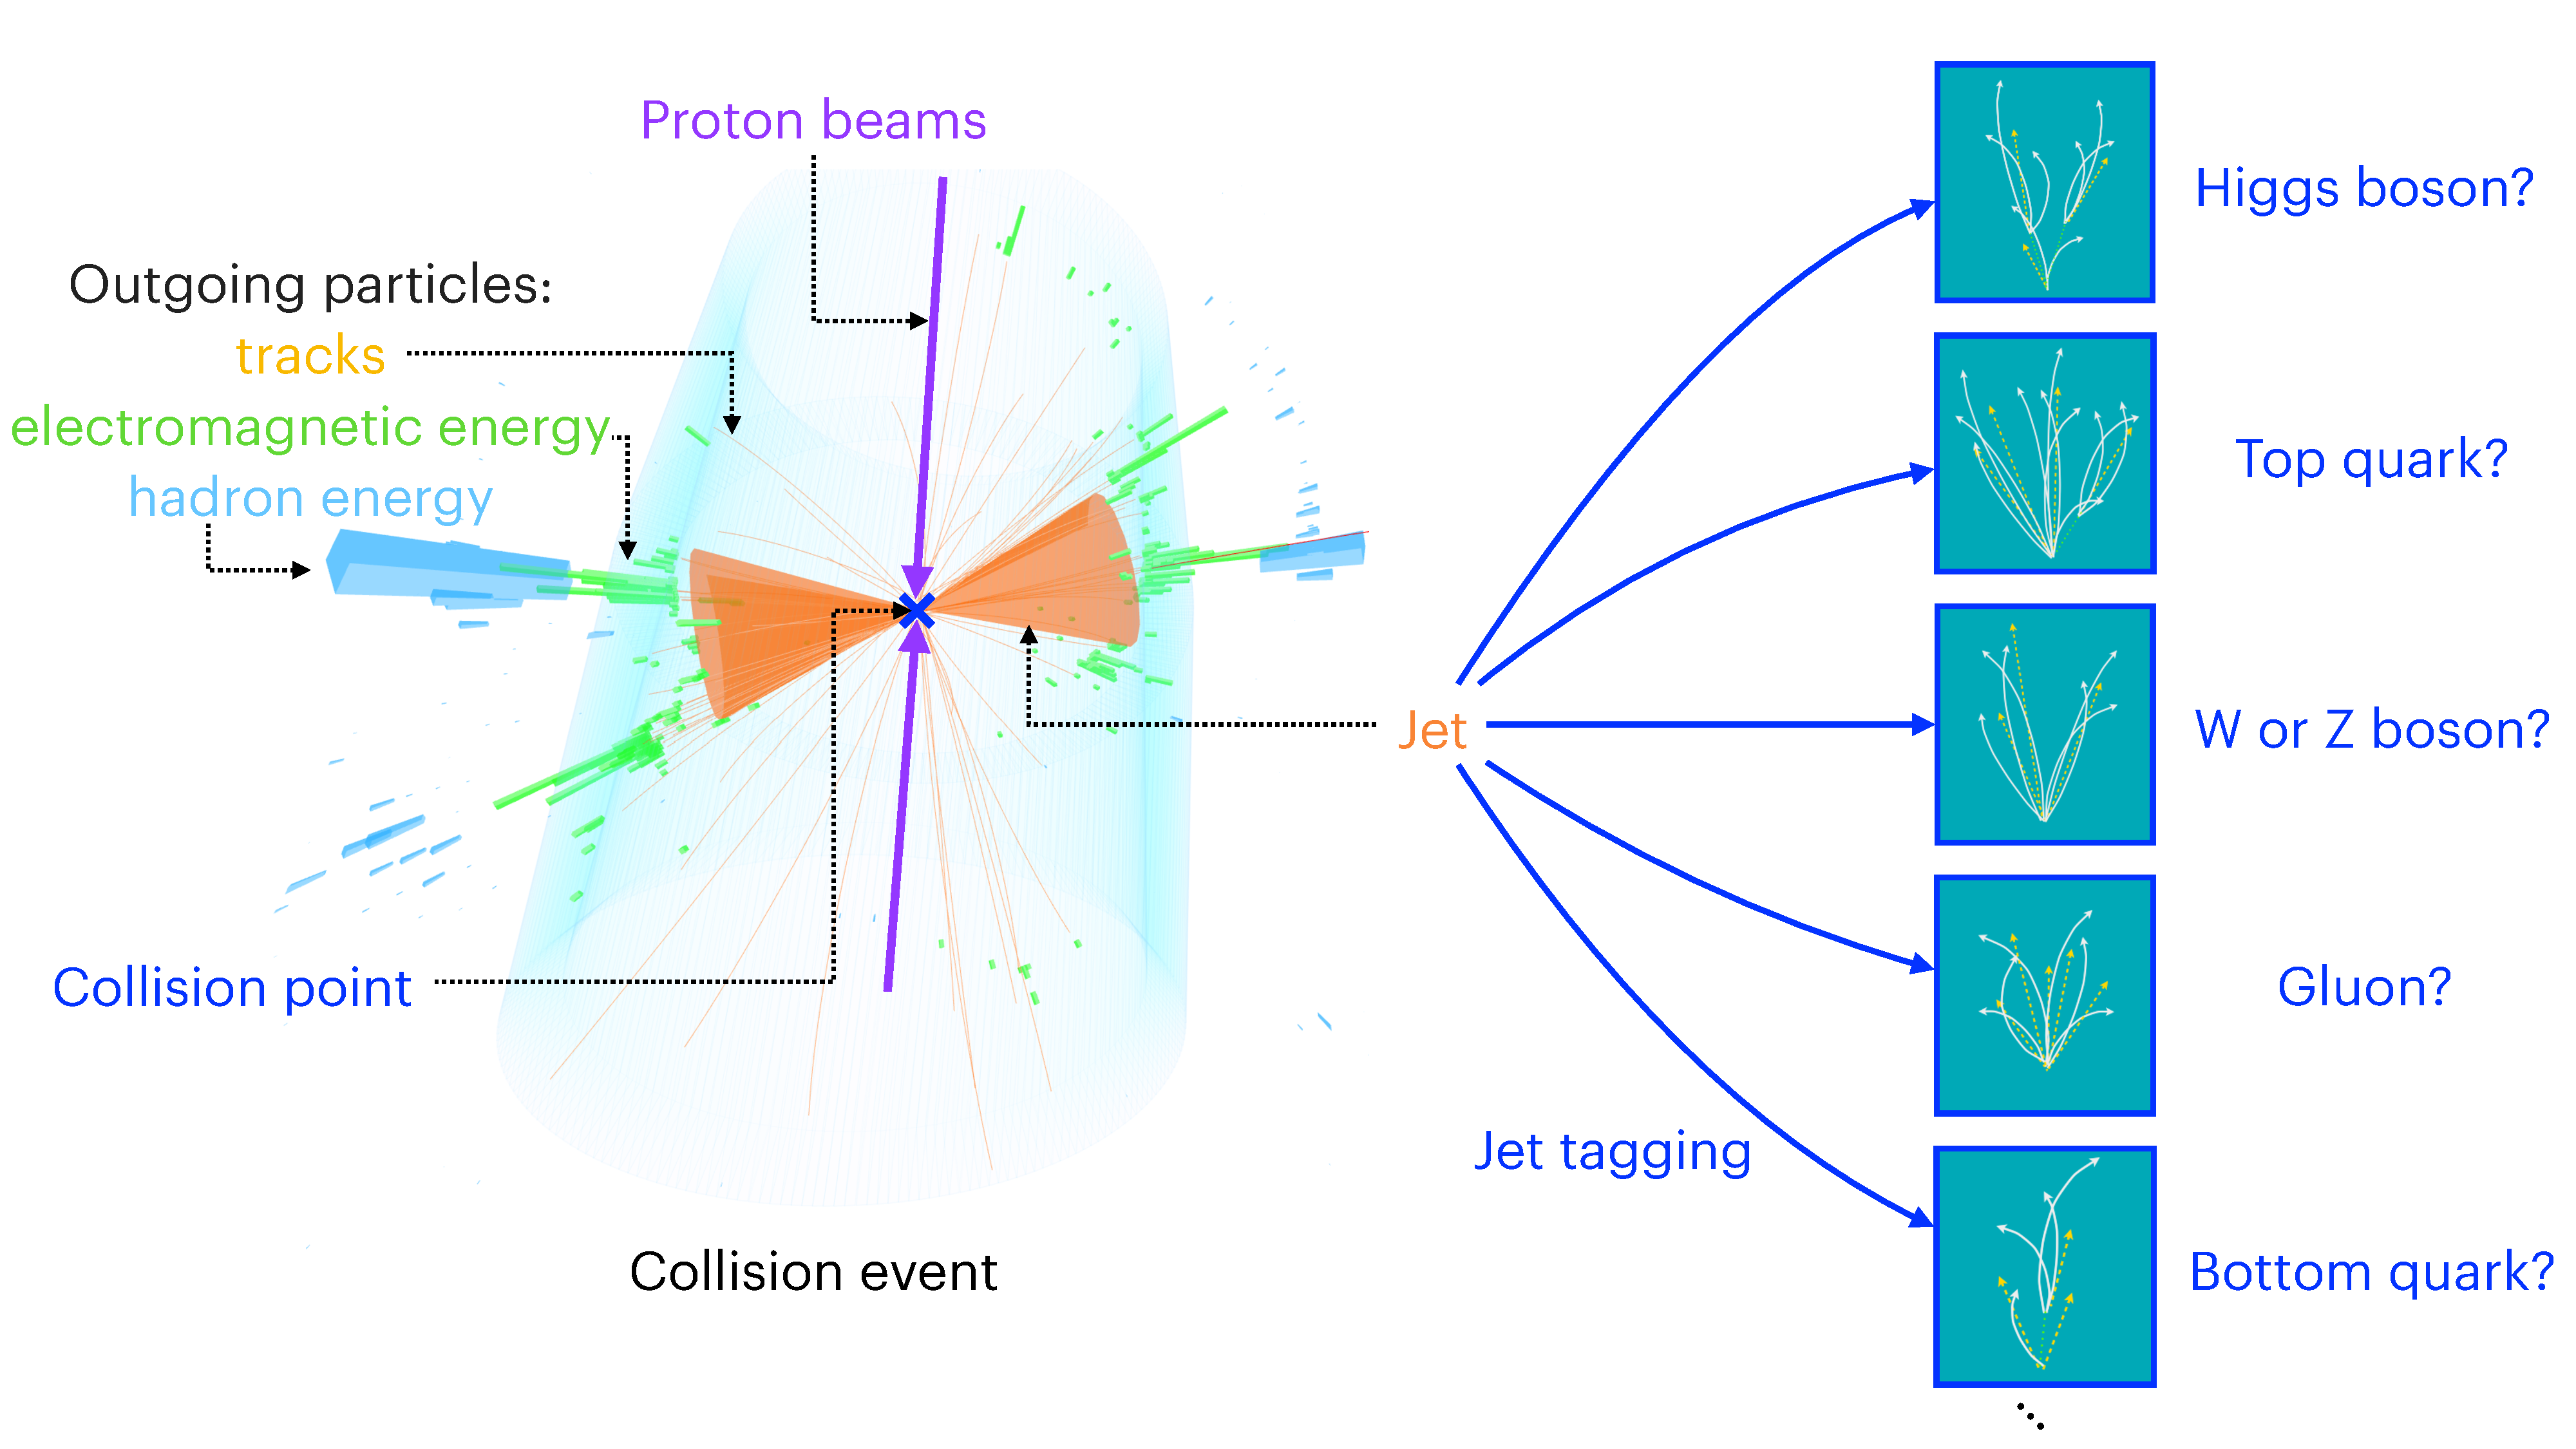
\includegraphics[width=0.9\textwidth]{jet_tagging.pdf}
    \caption[Jet tagging]{
        A visual representation of a collision event at the LHC and the task of jet tagging~[\myextcite{Duarte:2024xkc}].
        Proton beams (purple arrows) cross at a collision point (blue cross).
        Outgoing particles make tracks (curved orange lines), energy deposits in the electromagnetic calorimeter (green boxes), and energy deposits in the hadron calorimeter (blue boxes).
        The orange cone represents a cluster of tracks and energy deposits reconstructed as a jet.
        The task of jet tagging is to infer, on a statistical basis, the origin of a jet based on its measured characteristics.
        \label{fig:jet_tagging}
    }
\end{figure}

At the LHC, large detectors are situated around collision points to observe the remnants of the collisions.
We do not directly observe the outgoing particles from these collisions, instead we can only measure the signals created in these detectors by the stable particles as they pass through them.
For example, and silicon-based tracking devices measure the positions of hits created by charged particles along their trajectory, and calorimeters measure the energy deposited by these particles.
The distillation of the raw detector data into a physics-centric particle-level representation is called \emph{reconstruction}, and is traditionally done in multiple stages at different levels of abstraction.
Moreover, to ensure a high likelihood of a high-energy collision, large ``bunches'' of protons are collided.
This has the side effect of creating multiple, nearly simultaneous low-energy collisions, whose remnants overlap with those of the high-energy collision that we're interested in studying.
This phenomenon, called \emph{pileup}, complicates the reconstruction process, and mitigation of the effects of pileup is of prime importance.

Due to the staggering data rates produced by the 40 million collisions per second at the LHC, it is impossible to record and analyze every single collision.
Instead, the CMS experiment relies on the real-time event filter system, built from custom hardware and field-programmable gate arrays (FPGAs) and known as the \emph{trigger}, to reduce these data rates to a manageable level.
A crucial constraint is that the decision of whether to save or discard an event must be made in less than about 10 microseconds.
The main challenge is to do this reduction without rejecting collision events resulting from rare processes that we would like to study.

I analyze petabytes of proton-proton collision data to disentangle rare signal processes from the background to measure the properties and interactions of subatomic particles.
To enable this work, I develop algorithms based on artificial intelligence (AI) and machine learning (ML) to analyze the high-dimensional data from the detectors and classify or reconstruct particles or jets in these collision events.
My research focuses on
(R1) measurements of Higgs bosons decaying to quarks with high \pt,
(R2) searches for exotic new physics involving jets and long-lived particles (LLPs),
(R3) developing novel AI and ML algorithms for event reconstruction and simulation to enable these physics results, and
(R4) developing methods to accelerate AI algorithm training and inference (i.e., execution), e.g., to improve the real-time LHC event selection in the trigger.
This work is naturally interdisciplinary, at the interface of physics, computer science, AI, and electrical engineering.
My research also crosses traditional academia/industry divides, and I have collaborated with computer scientists and engineers.

In recognition of my work, I have received the APS Henry Primakoff Award for Early-Career Particle Physics in 2024, Sloan Research Fellowship in 2023,and RCSA Cottrell Scholar Award in 2023.
Along with the rest of CMS, ATLAS, LHCb, and ALICE Collaborations, we were awarded the 2025 Breakthrough Prize in Fundamental Physics for detailed measurements of Higgs boson properties confirming the symmetry-breaking mechanism of mass generation and the exploration of nature at the shortest distances and most extreme conditions at the LHC.
I have also been invited to give keynote presentations at the International Conference on Machine Learning (ICML) and the International Conference on High Energy Physics (ICHEP) in 2024 and Machine Learning for Jets (ML4Jets) in 2025.

\vspace{-1ex}
\subsubsection*{R1. High-\pt Higgs boson measurements}

On July 4, 2012, the discovery of a new fundamental particle, the Higgs boson (\PH), was announced by the ATLAS and CMS Collaborations.
This discovery confirmed the existence of a new kind of field, known as the Higgs field, whose physical incarnation is the Higgs boson.
Measuring the Higgs boson's interactions is necessary to confirm the validity of the SM, and any deviations may give a critical hint for new laws of physics.
To measure these interactions, we look for the Higgs boson in a multitude of production and decay processes, each one with a complementary sensitivity to a different set of couplings depending on the participating particles.
For example, measuring the rate of Higgs boson pair ($\PH\PH$) production enables us to constrain, and ultimately determine, the Higgs boson self-interaction strength $\kappa_\lambda$ as well as the interaction strength between two vector bosons and two Higgs bosons $\kappa_{2\PV}$.
For example, the connection between measuring the rate of vector boson fusion $\PH\PH$ production and the $\kappa_{2\PV}$ coupling modifier is illustrated in Fig.~\ref{fig:higgs}.

\begin{figure}[htpb]
    \centering
    \includegraphics[width=0.8\textwidth]{VBFHH4b.pdf}
    \caption[Higgs boson pair production]{
        Diagram for Higgs boson pair production through vector boson fusion (upper right).
        Measuring this process enables us to constrain $\kappa_{2\PV}$ shown in red.
        Candidate event in CMS of highly energetic $\PH\PH$ production via vector boson fusion (lower left)~[\myextcite{CMS-PAS-HIG-23-012}].
        The two large-radius jets (orange cones) are consistent with the decay of two Higgs bosons, and the two small-radius jets (yellow cones) are consistent with the two forward jets expected from vector boson fusion.
        \label{fig:higgs}
    }
\end{figure}

Without an increase in the center-of-mass collision energy, the improvement in the LHC's sensitivity is limited if we only repeat established searches on larger data sets.
Therefore, innovation and developing new search strategies are necessary.
At high-\pt, the decay products of the Higgs boson merge into a single large-radius jet, as shown in Fig.~\ref{fig:merged}.
Exploiting this merged final state and developing ML algorithms to identify it has proven to be one of the most fruitful new strategies.

\begin{figure}[htbp]
    \centering
    \includegraphics[width=0.4\textwidth]{PersonalStatement2022_figures/CMS-HIG-20-011_Figure_005-b.pdf}
    \includegraphics[width=0.4\textwidth]{PersonalStatement2022_figures/CMS-HIG-20-011_Figure_006-c.pdf}
    \includegraphics[width=0.4\textwidth]{PersonalStatement2022_figures/CMS-HIG-24-010_Figure_024-a.pdf}
    \includegraphics[width=0.4\textwidth]{PersonalStatement2022_figures/CMS-HIG-20-011_Figure_007-a.pdf}
    \caption[HH4b and HHbb4q final states]{
        Merged $\PH\PH\to4\PQb$ (upper left) and merged $\PH\PH\to\bbbar\PW\PW\to\bbbar 4\Pq$ (upper right) final states~[\myextcite{CMS:2025ngq}].
        The data and fitted signal and background distributions are shown for the gluon fusion category in the Run~3 high-$\pt$ $\PH\PH\to 4\PQb$ (lower left) and the Run~2 high-$\pt$ $\PH\PH\to\bbbar\PW\PW\to\bbbar 4\Pq$ search (lower right).
        The lower panel shows the ratio of the data and the total prediction, with its uncertainty represented by the shaded band.
        The error bars on the data points represent the statistical uncertainties.
        \label{fig:merged}
    }
\end{figure}

My previous work within the CMS Collaboration published in \emph{Phys. Rev. Lett.} established for the first time the high-\pt, merged $\PH\PH\to4\PQb$ final state as one of the most sensitive channels using Run~2~[\myextcite{CMS:2022nmn}].
To improve the sensitivity of this search with Run~3 data, my former graduate student Raghav Kansal and I along with CMS collaborators developed a ``global particle transformer'' algorithm to classify a highly granular multitude of jet types, as shown in Fig.~\ref{fig:glopart}~[\myextcite{Li:2024htp}, \myextcite{CMS:2026uph}].
This builds on my prior work on one of the first graph neural networks (GNNs) for jet tagging~[\myextcite{Moreno:2019bmu}, \myextcite{Moreno:2019neq}].
The global particle transformer algorithm provided a 25\% signal efficiency improvement compared to the previous algorithm for the same background rate and it is widely used in CMS.
With this improvement, my graduate student Daniel Primosch and I along with collaborators led a search for $\PH\PH\to4\PQb$ production through gluon fusion and vector boson fusion with Run-3 data recently submitted to \emph{Phys. Rev. D}~[\myextcite{CMS:2026znu}].
We also collaborated to implement the statistical combination of the best results from the Run~3 and Run~2 $\PH\PH\to4\PQb$ searches to further improve the sensitivity to $\kappa_\lambda$ and $\kappa_{2\PV}$---advancing our knowledge of the allowed range for these fundamental parameters.

\begin{figure}[htbp]
    \centering
    \includegraphics[width=0.8\textwidth]{CMS-JME-25-001_Figure_001.pdf}
    \includegraphics[width=0.8\textwidth]{CMS-JME-25-001_Figure_002.pdf}
    \caption[Global particle transformer]{
        Diagram of the global particle transformer model architecture (upper)~[\myextcite{CMS:2026uph}].
        The model processes two different sets of input features per jet, from particle candidates and secondary vertices.
        Pairwise features are also calculated between each input element.
        Full suite of jet types considered for the first version of the global particle transformer multiclass classification task (lower).
    }
    \label{fig:glopart}
\end{figure}


After the decay to bottom quarks, the next most prominent decay mode of the Higgs boson is its decay to two \PW bosons ($\PH\to\PW\PW$).
This final state is experimentally challenging to identify reliably, especially when the $\PW$ bosons decay to quarks, but can improve the sensitivity to Higgs couplings.
My former graduate student Raghav Kansal was the main analyst for a search for Higgs boson pair production through gluon fusion and vector boson fusion in the $\PH\PH\to\bbbar\PW\PW\to\bbbar 4\Pq$ all-hadronic final state.
This search also used one of the first the transformer-based algorithm to identify the Higgs boson decay, and was one of the most sensitive in CMS to the coupling between two vector bosons and two Higgs bosons $\kappa_{2\PV}$~[\myextcite{CMS-PAS-HIG-23-012}].
Together with other CMS collaborators, I contributed to the combination of all Run~2 Higgs boson pair producerion searches using Run~2 data, which included this channel, and was submitted to \emph{J. Phys. G.}~[\myextcite{CMS:2025ngq}].
Finally, the same techniques were applied to search for heavy scalar resonance \PX decaying to a Higgs boson (\PH) and a Higgs-like scalar boson (\PY) in the two bottom quark ($\PH\to\bbbar$) and four quark ($\PY \to \PV\PV \to 4\Pq$) final state in a manuscript recently submitted to \emph{J. High Energy Phys.}~[\myextcite{CMS:2026shw}].
These searches formed a major part of Raghav Kansal's Ph.D. thesis, which he defended on June 18, 2024.

While measuring the Higgs boson pair production can probe the trilinear self-interaction, which is the interaction between three Higgs bosons, it does not directly probe the quartic self-interaction, which is the interaction between four Higgs bosons.
To access the quartic self-interaction, we need to search for the production of three Higgs bosons, which is even rarer than pair production.
This further exacerbates a combinatorial challenge known as the \emph{jet assignment problem}: assigning jets to Higgs boson candidates.
The complexity of this challenge increases when simultaneously considering multiple reconstruction possibilities, i.e., a single Higgs boson can produce two ``resolved'' small-radius jets each containing a shower initiated by one \PQb quark or one ``merged'' large-radius jet containing a merged shower initiated by a \bbbar pair.
My graduate student Haoyang (Billy) Li led a project generalizing symmetry-preserving attention networks (SPANets) to address this challenge.
With this ML approach, the fraction of correctly matched Higgs bosons increased by more than a factor of two with the ML approach compared to traditional approaches, as shown in Fig.~\ref{fig:hhh}.
This work was published in \emph{J. High Energy Phys.}~[\myextcite{Li:2024qfq}].
A version of this algorithm has been adopted in the first CMS search for triple Higgs boson production, which we co-authored and will be submitted to \emph{Phys. Rev. Lett.} shortly~[\myextcite{CMS-PAS-HIG-24-012}].
The results of this search set the most stringent constraints to date on $\PH\PH\PH$ production and on the quartic self-interaction, while establishing a robust strategy for Higgs boson self-coupling measurements at the LHC and HL-LHC.

\begin{figure}
    \centering
    \includegraphics[width=0.43\textwidth]{2025-07-22_merged.pdf}
    \includegraphics[width=0.37\textwidth]{CMS-PAS-HIG-24-012_Figure_001-a.pdf}
    \caption[SPANet HHH reconstruction and search]{
        The performance of the enhanced SPANet algorithm that considers both resolved and merged jet reconstruction possibilities for $\PH\PH\PH$ production compared to the baseline (left)~[\myextcite{Li:2024qfq}].
        The reconstruction efficiency, defined as the fraction of the target Higgs bosons reconstructed by SPANet, is shown as a function of the target Higgs boson \pt.
        Post-fit yields in the CMS search for $\PH\PH\PH$ production signal-region categories with three reconstructed Higgs bosons (right)~[\myextcite{CMS-PAS-HIG-24-012}].
        Bins correspond to ten bins per category intervals of the SPANet score, ordered by increasing score.
        The expected $\PH\PH\PH$ contribution scaled up by a factor of 500 is shown in green.
        \label{fig:hhh}}
\end{figure}

Former graduate student Farouk Mokhtar led a search for high-$\pt$ $\PH\to\PW\PW\to\Pq\Pq\ell\nu$ production through gluon fusion and vector boson fusion, where both quarks and lepton are merged in a single jet.
This search was combined with a search in the all-hadronic channel and one focusing on $\PV\PH$ production in the one-lepton channel, and was recently submitted to \emph{J. High Energy Phys.}~[\myextcite{CMS:2026yrb}].
A significant novelty was the use of the transformer-based algorithm as a pre-trained model that was subsequently fine-tuned for the specific task of identifying the $\PH\to\PW\PW$ decay, while rejecting backgrounds that the model had not been trained on initially.
This fine-tuning approach was crucial for the sensitivity in the one-lepton channel, achieving 60\% greater signal efficiency than the baseline method without fine-tuning, as shown in Fig.~\ref{fig:hww}.
These measurements represent the first dedicated study of highly energetic $\PH\to\PW\PW$ decays, complementing earlier searches for high transverse momentum Higgs boson production in other decay channels and production processes led by my group~[\myextcite{Sirunyan:2017dgc}, \myextcite{Sirunyan:2020hwz}, \myextcite{CMS:2022wqf}, \myextcite{CMS:2024ddc}].
This search was a component of Farouk Mokhtar's Ph.D. thesis, which he defended on December 10, 2025.
This category of my research program was mainly supported by a DOE Early Career Award for ``Real-Time Artificial Intelligence for Particle Reconstruction and Higgs Physics'' (\$750,000 as sole PI, 2020--2025).
I also received a UCSD Academic Senate Research Grant for ``Transforming Higgs pair production searches at the LHC'' (\$15,000, 2025--2026).

\begin{figure}[h!]
    \centering
    \includegraphics[width=0.45\textwidth]{CMS-HIG-24-008_Figure_002-b.pdf}
    \includegraphics[width=0.45\textwidth]{CMS-HIG-24-008_Figure_006-f.pdf}
    \caption[HWW tagger performance]{
        Comparison of the tagger performance before and after fine-tuning (left).
        The data and fitted signal and background distributions are shown for the one-lepton category in the high-$\pt$ $\PH\to\PW\PW\to\Pq\Pq\ell\nu$ search (right).
        \label{fig:hww}
    }
\end{figure}

Finally, within the CMS Collaboration, I was selected to co-lead the Higgs $\bbbar$/$\ccbar$ Subgroup of the Higgs Physics Analysis Group from 2025 to 2027, responsible for coordinating and leading the development of analyses related to Higgs boson decays to bottom and charm quarks.

\vspace{-1ex}
\subsubsection*{R2. Exotic long-lived particle and jet-based searches}

Many BSM theories predict new particles with long lifetimes for several reasons, including approximate symmetries, small couplings between the LLP and lighter particles, and suppressed phase space available for decays.
For particles moving close to the speed of light, this can lead to macroscopic, detectable displacements between the production and decay points of an unstable particle with a proper decay length $c\tau \gtrsim 10\,\mu$m.
The experimental signatures of LLPs at the LHC are often very different from those of SM processes.
For example, LLP signatures can include deposits of energy inside the calorimeters without associated tracks, stopped particles that decay out of time with collisions, and displaced particle showers in the muon spectrometer.
While the unusual signatures of LLPs offer excellent prospects for their discovery at the LHC, standard reconstruction algorithms may reject events containing LLPs precisely because of their unusual nature.
These atypical signatures can also resemble noise, pileup, or misreconstructed objects in the detector, which may not be accurately modeled in simulations, necessitating data-driven methods to accurately estimate the backgrounds.

During this review period, my former postdoctoral fellow Dr. Daniel Diaz led a new search for LLPs using a data sample of $10^{10}$ decays of \PQb hadrons (hadrons that contain bottom quarks), which were recorded and ``parked'' for later analysis by CMS in 2018.
Data parking is a method to evade a major limitation of data collection at the LHC: the computational burden of immediately reconstructing every event.
Instead, raw data from these events were stored without further processing until the data taking run was complete and computational cores were less utilized.
This data set is especially sensitive to a class of models that predict that LLPs are produced in \PQb hadron decays with some small probability.
If the lifetime of the LLP is large enough, it can travel into the volume outside of the CMS tracker and calorimeters before decaying, producing a shower of hadrons leaving a high multiplicity of hits in the muon detectors, as shown in Fig.~\ref{fig:llp}.
Effectively, this approach uses the CMS muon detector system as a sampling calorimeter.
Building on our previous work searching for LLPs with this unique muon detector shower (MDS) signature~[\myextcite{CMS:2021juv}, \myextcite{CMS:2024bvl}, \myextcite{CMS:2024ake}], the new search targets similar hadronic decays of the LLP in the \PB parking data set.
The search, recently published in \emph{Phys. Rev. D}~[\myextcite{CMS:2025rtd}], yields the most stringent limits to date on the decay of a long-lived scalar particle to a pair of hadrons when the LLP is produced by a bottom hadron, particularly for long decay lengths.
% We have also contributed to several other searches for LLPs~[\myextcite{CMS:2022wjc}] and boosted dijet resonances~[\myextcite{CMS-PAS-EXO-24-007}].

\begin{figure}[h!]
    \centering
    \includegraphics[width=0.8\textwidth]{CMS-EXO-24-004_Figure.pdf}
    \caption[Example LLP signature]{
        Display of a candidate signal event in the \PB parking data set with an overlaid example diagram for the production of a pair of \PQb hadrons, where one decays to a kaon and the LLP $\Phi$.
        The display shows the hits (magenta points) in the muon endcap system that form the MDS cluster opposite the muon (red line), which is used to select the event online.
        Muon system chambers that recorded hits from a muon are shown as red rectangles.
        \label{fig:llp}
    }
\end{figure}

\vspace{-1ex}
\subsubsection*{R3. Novel machine learning for event reconstruction and simulation}

Within the CMS Collaboration, I was the co-leader of the Machine Learning Group from 2023 to 2025, responsible for benchmarking and validating ML methods, coordinating the integration and maintenance of ML software, monitoring the usage of ML in the collaboration, providing consulting, coordinating and centralizing ML training resources for newcomers, fostering ML R\&D, and reviewing publications on novel ML methods.
Under my leadership, CMS published four ML papers, and two more have been submitted for publication.
We also organized several hackathons, journal clubs, tutorials, and workshops on ML for the collaboration, including the ``CMS ML Hackathon: Anomaly Detection for Monitoring, Validation, and Discovery'' in July 2024.

Beyond the CMS Collaboration, my research includes developing new ML techniques to improve event reconstruction and simulation in particle physics.
This work is done in collaboration with a relatively small number of coauthors and I made significant technical and writing contributions to these papers.
A novel ML algorithm I helped develop in Ref.~[\myextcite{Pata:2021oez}], published in \emph{Eur. Phys. J. C}, uses a ML to improve the particle-flow (PF) algorithm, known as the MLPF.
Traditionally, the PF algorithm correlates tracks and calorimeter energy clusters from different detector layers using a set of ad-hoc rules to reconstruct charged and neutral hadron candidates as well as photon, electron, and muon candidates with high efficiency and good energy resolution.
While this approach is effective, it can be brittle and difficult to maintain as detector responses change or detectors get upgraded.
Our ML-based method distills this logic into an algorithm that can be easily updated by retraining on new data or simulation, and gives speed improvements by parallelizing its computation.

In previous work, we have shown this approach can be extended to future proposed colliders and detectors, such as the Compact Linear Collider (CLIC), in work published in \emph{Comm. Phys.}~[\myextcite{Pata:2023rhh}].
We also studied the applicability of new hardware for accelerated ML training and inference, like the SDSC Voyager supercomputer composed of AI-specific Intel Habana Gaudi and Goya processors.
This work is facilitated by the NSF award  ``Category II: Exploring Neural Network Processors for AI in Science and Engineering'' (\$5,000,000 for SDSC, 2020--2026) for which I am a co-PI.

During this review period, we demonstrated the cross-detector transfer learning capabilities of MLPF by pre-training the model on one collider and detector design, and subsequently fine-tuning the model for a different collider and detector design.
With an order of magnitude fewer samples from the second dataset, we achieved a comparable performance to costly training from scratch, as shown in Fig.~\ref{fig:mlpf}, opening the door to rapid detector design and optimization using ML.
This work was published in \emph{Phys. Rev. D} with former graduate student Farouk Mokhtar as first author~[\myextcite{Mokhtar:2025zqs}].
In addition, we evaluated the performance of the MLPF algorithm in real CMS data and simulation for the first time in a paper submitted to \emph{J. High Energy Phys.}~[\myextcite{CMS:2026znb}].
These results indicate that the MLPF algorithm can match or improve on the existing PF algorithm, while being more parallelizable and portable to heterogeneous computing accelerators like GPUs.

\begin{figure}[h!]
    \centering
    \includegraphics[width=0.4\textwidth]{scaling_jetperf.pdf}
    \includegraphics[width=0.4\textwidth]{CMS-PFT-25-001_Figure_010-c.pdf}
    \caption[MLPF performance]{
        The jet energy resolution as a function of the fine-tuning dataset size, for the fine-tuned MLPF model (orange), a model trained from scratch (blue), and the traditional PF algorithm (grey) in electron-positron collisions~[\myextcite{Mokhtar:2025zqs}].
        The fine-tuned model is able to outperform PF with a much smaller dataset size compared to the from-scratch model.
        The runtime of the baseline PF reconstruction compared to the MLPF inference, demonstrating the improved computational performance of MLPF in CMS software (right)~[\myextcite{CMS:2026znb}].
    }
    \label{fig:mlpf}
\end{figure}

A related line of work is to develop foundation models (FMs), which are large-scale ML models pre-trained using massive unlabeled data sets, for high energy physics (HEP).
Typically, these models are first pre-trained in a self-supervised way on an unlabeled dataset then fine-tuned on a labeled dataset for different downstream tasks, such as jet classification, as shown in Fig.~\ref{fig:hepfm}.
We have studied and developed different pre-training strategies based on scaling up a simple framework for contrastive learning of representations (SimCLR)~[\myextcite{Zhao:2024kry}], training a fine-griained classifier~[\myextcite{Li:2024htp}], and a joint-embedding predictive architecture (JEPA), which predicts representations of ``masked'' particles inside a jet using the surrounding particles as the context~[\myextcite{Katel:2024ygn}].
With collaborators, I also contributed to developing a contrastive learning approach based on different jet clustering algorithms and the renormalization group~[\myextcite{Hao:2025abk}].
We have also studied efficient and interpretable algorithms based on transformers for charged particle tracking~[\myextcite{Miao:2024oqy}, \myextcite{Govil:2025nvy}] and jet tagging~[\myextcite{Bhatnagar:2024fkx}, \myextcite{Legge:2025cnm}, \myextcite{Wang:2025dky}, \myextcite{Wang:2026lqb}].
Several of these works have been accepted at ICML and the Machine Learning and the Physical Sciences Workshop at the Neural Information Processing Systems (NeurIPS) conference.
This research was supported by my Cottrell Scholar Award (\$100,000, 2023--2026) and Sloan Research Fellowship (\$75,000, 2023--2025).

\begin{figure}[h!]
    \centering
    \includegraphics[width=0.7\textwidth]{HEPFM.pdf}
    \caption[Foundation model for HEP]{Schematic of a foundation model based on HEP data~[\myextcite{Duarte:2025qbk}].
        Data is used to pre-train a large model, which can then be fine-tuned (or adapted) to various downstream tasks.}
    \label{fig:hepfm}
\end{figure}

My group and I have worked on developing anomaly detection algorithms for particle physics.
An anomaly, in this case, refers to a collection of events that share unusual characteristics that are potentially inconsistent with SM processes, and thus may be related to new BSM particles or interactions.
The methods I've developed are mainly based on autoencoders, a type of ML algorithm trained on SM-like data that compresses then decompresses input data and measures the level of disagreement between the output and the input.
A large discrepancy indicates the data is unlike the SM-like data seen during training, and may be an anomalous signal.
Postdoctoral fellow Melissa Quinnan, graduate student Ellison Scheuller, and I have helped implement this anomaly detection algorithm into data-taking during LHC Run 3~[\myextcite{CMS-DP-2023-079}, \myextcite{CMS-DP-2024-059}, \myextcite{CMS-DP-2025-061}] based on prior work published in \emph{Nat. Mach. Intell.}~[\myextcite{Govorkova:2021utb}].
Previously, with former undergraduate student Zichun Hao and former graduate student Raghav Kansal, we developed the first Lorentz-equivariant autoencoder for particle physics published in \emph{Eur. Phys. J. C}~[\myextcite{Hao:2022zns}].

High energy physicists rely heavily on simulation for a wide array of tasks, including data selection, statistical inference, and design optimization for new experiments.
However, the computational demands for simulation of current and next generation experiments are so immense that they have inspired the investigation of generative ML models to decrease simulation time while maintaining fidelity.
Usually, the most computationally intensive step of the simulation is the modeling of the interactions between particles and the detector material.
Some of my work is focused on developing generative ML models using GNNs to improve or speed up this computationally expensive simulation.
Building on our previous work in the 2021 NeurIPS conference~[\myextcite{Kansal:2021cqp}], we have developed a new more efficient transformer-based generative algorithm and comprehensive metrics to compare them, in work published in \emph{Phys. Rev. D}~[\myextcite{Kansal:2022spb}].
A workshop paper describing the improved efficient algorithm was also accepted to the NeurIPS Workshop on Machine Learning and the Physical Sciences in 2023~[\myextcite{Li:2024xpw}].
The software related to this work was released as a public library called JetNet, described in a publication in \emph{J. Open Source Softw.}~[\myextcite{Kansal:2023joss}].

A common thread throughout this work is developing open, public scientific data sets~[\myextcite{Chen:2021euv}] and sharable AI models following the findable, accessible, interoperable, and reusable (FAIR) principles~[\myextcite{Duarte:2022job}].
These principles are significant because they enable more reproducible science, greater access to a larger community of researchers, and support educational efforts.
This work was partially funded by a DOE award \href{https://fair4hep.github.io}{``FAIR4HEP: FAIR Framework for Physics-Inspired AI in High Energy Physics''} (\$2,250,000 total, \$450,000 for UCSD, 2020--2023) on which I was a co-PI.

\vspace{-1ex}
\subsubsection*{R4. Accelerated machine learning for trigger and computing}

In the next phase of the LHC starting in 2030, the instantaneous luminosity will increase by a factor of five and the CMS detector will become more complex, producing up to hundreds of terabytes of data per second.
This avalanche of data must be filtered down by several orders of magnitude by the real-time, hardware-based trigger system within microseconds using field-programmable gate arrays (FPGAs), as shown in Fig.~\ref{fig:trigger}.
To meet this challenge, my research focuses on developing new ultra-low-latency AI techniques trained to reconstruct, identify, and preserve these precious collisions.
This work has broader impacts for many disciplines, including multimessenger astronomy, neutrino physics, neuroscience, and microscopy~[\myextcite{Deiana:2021niw}, \myextcite{Duarte:2022efficient}].


\begin{figure}[htpb]
    \centering
    \includegraphics[width=0.8\textwidth]{LHC_Event_Processing.pdf}
    \caption{Flowchart of LHC event processing after the high-luminosity upgrade in 2030.
        Collisions occur at a rate of 40 MHz, and the two-tier trigger system must reduce this to a manageable rate of 7.5 kHz for storage and offline analysis.
        The first level of the trigger (L1) is implemented in custom hardware, including FPGAs, and must make decisions within 12.5 microseconds, reducing the rate to 750 kHz.
        The second level of the trigger (HLT) is implemented in software running on a CPU farm equipped with GPUs and has a latency of around 3--4 seconds, further reducing the rate to 7.5 kHz.
    }
    \label{fig:trigger}
\end{figure}

I contributed to the design, implementation, and evaluation of real-time AI algorithms on FPGAs and ASICs for the LHC trigger and data acquisition~[\myextcite{Gonski:2026jgu}].
While FPGAs and ASICs deliver high performance and energy efficiency for such workloads, their development remains complex and requires significant expertise.
My key contribution is the creation~[\myextcite{Duarte:2018ite}] and continued development~[\myextcite{Schulte:2025mai}] of \texttt{hls4ml}, a flexible, open-source platform for converting high-level neural networks from PyTorch, Keras, or similar frameworks into high-level synthesis (HLS) kernels suitable for deployment on FPGAs and ASICs.
\texttt{hls4ml} is structured in a modular fashion, following the design of modern compilers, as shown in Fig.~\ref{fig:hls4ml_flow}.
The final hardware design is obtained by composing templated implementations of the optimized operators, which can be configured to balance between latency and resource consumption.
When synthesizing the hardware, hls4ml abstracts the interaction with vendor-specific tools, automating synthesis, placement, and routing, allowing users to generate a deployable bitstream in a few lines of Python code.
This library has been widely adopted by the particle physics community and beyond, with over 2000 stars on GitHub and more than 800 citations in the literature.

\begin{figure}[htpb]
    \centering
    \includegraphics[width=0.6\linewidth]{hls4ml_flow.pdf}
    \caption[hls4ml model conversion flow]{\texttt{hls4ml} model conversion flow: Models from supported frameworks are first translated into a unified intermediate representation (IR), which captures the computation graph and layer configurations independently of the model framework or target hardware.
        The IR then undergoes a series of hardware-aware optimizations, including precision adjustment, data layout transformation, and operator fusion, producing a computation graph optimized for dataflow inference on the target platform.
    }
    \label{fig:hls4ml_flow}
\end{figure}

Recently, we developed new FPGA implementations of deep sets and graph neural networks for jet tagging in the LHC trigger, and compared their performance~[\myextcite{Odagiu:2024bkp}].
This work has been used to develop the next generation of jet tagging algorithms for the upgraded CMS Level-1 trigger to be deployed in LHC Run 4 starting in 2030.
% In Ref.~[\myextcite{Shenoy:2023ros}], we developed a differentiable approximation to the Earth mover's distance in order to train a better autoencoder for data compression in real time for an LHC detector.

With tools like \texttt{hls4ml} that make deployment of ML models on FPGAs and ASICs more accessible, there is a growing desire to automate the process of design space exploration and neural architecture search (NAS) for ML models in order to optimize their performance on these platforms.
My graduate student Jason Weitz led a project to develop a neural architecture codesign (NAC) tool, which combines NAS and network compression in a two-stage approach to discover hardware efficient models.
This approach was demonstrated on various tasks, including Bragg peak finding and jet classification, achieving models with improved accuracy, smaller latencies, or reduced resource utilization, quantified through a proxy metric known as bit operations (BOPs), relative to the baseline models~[\myextcite{Weitz:2025tcj}].
Recently, the approach has been extended to better quantify the hardware costs in terms of lookup tables, DSPs, flip-flops, BRAM, and latency.
Specifically, the Surrogate Neural Architecture Codesign Package (SNAC-Pack)~[\myextcite{Weitz:2025dia}] runs a multi-objective parallelized search using a hardware surrogate model, known as \texttt{wa-hls4ml}~[\myextcite{Hawks:2025hew}], which outputs per-trial resource and latency estimates, avoiding the synthesis cost that would otherwise dominate the search loop.
% An agentic frontend lets users run the pipeline on new datasets without modifying the framework.
SNAC-Pack was demonstrated on a qubit readout task, reducing the design space exploration process from months of manual fine-tuning to hours of automated search.

With collaborators in the CSE Department and led by graduate student Olivia Weng, we have developed efficient hardware implementations of neural networks with skip connections~[\myextcite{Weng:2023tailor}], improved the robustness of neural networks to faults induced by radiation~[\myextcite{Weng:2024fkeras}], and implemented ensembles of neural networks as lookup tables to improve their scalability~[\myextcite{Weng:2025amigolut}].
% For all the above work, I oversaw the development and validation of these implementations and cowrote the publications.

As more physics reconstruction and simulation algorithms turn to ML-based approaches, there is a need to scale up and accelerate the inference of large ML models in order to run them on billions of collision events in distributed computing workflows.
The goal is to enable the use of alternative processors, alongside traditional CPUs, that are better adapted to highly parallelizable ML inference workloads in a scalable way.
With coauthors, we developed a new framework of ``ML inference as a service'' for particle physics~[\myextcite{Duarte:2019fta}], in which heterogeneous computing elements, including graphics processing units (GPUs), FPGAs, and AI-targeted application-specific integrated circuits (ASICs), can be flexibly composed and used with in tandem with CPUs.
I contributed to the integration of these workflows into the CMS computing framework, which is documented in a paper pulished in \emph{Comput. Softw. Big Sci.}~[\myextcite{CMS:2024twn}].
We also recently developed a framework for deploying the necessary server infrastructure as a GPU-equipped Kubernetes cluster~[\myextcite{Kondratyev:2025jfj}].

This work was also supported by my DOE Early Career Award and the \href{https://a3d3.ai}{``NSF Harnessing the Data Revolution (HDR) Institute for Accelerated AI Algorithms for Data Driven Discovery (A3D3)''} (\$15,000,000 total, \$675,600 for UCSD, 2021--2026) focused on the domains of multimessenger astronomy, neuroscience, and particle physics.
For this Institute, I am a key personnel, the UCSD institute PI and co-chair of the Equity and Career Committee.
Some of this work is also supported by a DOE Award for ``Real-time Data Reduction Codesign at the Extreme Edge for Science'' (\$750,000 total, \$225,000 for UCSD, 2021--2024), on which I am a co-PI.
Finally, I am a key personnel on a DOE award ``UCSD Experimental and Theoretical Particle Physics'' (\$6,928,000 total, \$3,915,000 for four faculty members in the UCSD CMS group, 2024--2028)

\vspace{-1ex}
\subsection*{Mentorship}

My research group includes two postdoctoral fellows, Dr. Melissa Quinnan and Dr. Farouk Mokhtar, seven physics graduate students, Anthony Aportela (Ph.D., year 6), Daniel Primosch (Ph.D., year 6), Russell Marroquin Solares (Ph.D., year 4), Zihan Zhao (Ph.D., year 4), Haoyang (Billy) Li (Ph.D., year 4), Jason Weitz (Ph.D., year 2), and Ellison Schueller (Ph.D., year 2), and more than 10 undergraduate student researchers.
I also supervised or co-supervised several Computer Science and Engineering (CSE) and Electrical and Computer Engineering (ECE) graduate students: Olivia Weng (CSE Ph.D., year 6, co-supervisor with Ryan Kastner).
With my support, several members of my group have received significant awards and funding.
For example, Melissa Quinnan was named an LPC Distinguished Researcher in 2026, and Jason Weitz and Ellison Schueller were both awarded fellowships from the Western Advanced Training for Computational High-Energy Physics (WATCHEP) for 2025--2027 and 2026--2028, respectively.
From the School of Physical Sciences, Timothy Legge, Dmitri Demler, and Jet Yue were awarded Dean's Undergraduate Awards for Excellence in 2024--2025 or 2025--2026.
Many other undergraduate students have also received awards and funding from the UCSD TRELS program, Undergraduate Research Hub, the Division of Physical Sciences Undergraduate Research Award, and NSF IRIS-HEP.
A great deal of the work done by undergraduates in my group has led to publications or conference papers.
% This includes work led by Rohan Shenoy on improved autoencoder training~[\myextcite{Shenoy:2023ros}], Anni Li on simulation~[\myextcite{Li:2024xpw}] and Zichun Hao on Lorentz-equivariant autoencoders for anomaly detection~[\myextcite{Hao:2022zns}], and Jason Weitz and Dmitri Demler on neural architecture codesign~[\myextcite{McDermott:2023neural}].

Previously, my graduate students Anthony Aportela and Russell Marroquin Solares received HEPCAT and WATCHEP fellowships, respectively.
The HEPCAT fellowship is supported by a DOE award (\$3,700,000 total, \$110,000 for UCSD so far, 2021--2026), which aims to support and train the next generation of HEP instrumentation researchers.
For this award, I am Key Personnel and lead the \href{https://hepcat.ucsd.edu/topical-groups/tg7-ai-ml-for-detectors-2/}{Topical Group on AI/ML for detectors}.
The WATCHEP fellowship is also supported by a DOE award (\$2,000,000 total, \$440,00 for UCSD, 2022--2027), which trains students on computational topics in experimental particle physics.

Although outcomes of mentorship can be difficult to quantify, many of my trainees have gone on to begin successful careers in academia and industry, including prestigious Schmidt AI and CERN Fellowships, as shown in Table~\ref{tab:alumni}.

\begin{table}[htpb]
    \centering
    \caption{Graduate student and postdoctoral trainees and their positions after training.}
    \begin{tabular}{ll}
        Trainee         & Position after training                                    \\\hline
        Raghav Kansal   & Schmidt AI Postdoctoral Fellow, Caltech/Fermilab           \\
                        & $\to$ Senior Deep Learning Scientist, Bexorg, Inc.         \\
        Farouk Mokhtar  & CERN Fellow in Applied Physics                             \\
        Daniel Diaz     & Computational Data Science and Research Specialist 3, SDSC \\
        Melissa Quinnan & CERN Fellow in Experimental Physics                        \\
    \end{tabular}
    \label{tab:alumni}
\end{table}

\vspace{-1ex}
\subsection*{Teaching}

My teaching approach is to foster an inclusive, welcoming learning environment and promote active learning through evidence-based methods.
My most significant contributions to teaching are the creation and modernization of several upper-division computational physics courses, including one focused on machine learning in physics.
I strive to provide sufficient scaffolding through lower-stakes, incremental assignments.
However, given the ubiquity and popularity of AI tools, I have recently shifted to focus more on in-class assessments and projects, which are more difficult to outsource to AI, and less on homework assignments.
I also use ``exit tickets'' and surveys to collect feedback on the course structure, difficulty of projects, and appropriateness of the assessments.

I created a new introductory graduate and upper-division undergraduate course, currently taught as a special topics course called Physics 139/239: Machine Learning in Physics, which I have now taught three times (Winter 2023, Spring 2024, and Fall 2025).
The course structure consists of weekly lectures on conceptual topics, e.g. statistics, linear algebra, scientific data set exploration, feature engineering, (stochastic) gradient descent, neural networks, and unsupervised learning.
Students learn key concepts in data science and machine learning, including selecting and preprocessing data, designing machine learning models, evaluating model performance, and relating model inputs and outputs to the underlying physics concepts.
They apply these methods to the domains of collider physics, neutrino physics, astronomy, and others.
In addition to hands-on programming-based homework assignments, the final project for the course is an open-ended group research project to reproduce the results of an ML in physics research article, with intermediate checkpoints to provide feedback.
A midterm assignment to propose the project is also required.
The projects use real, open scientific datasets, including those shown in Fig.~\ref{fig:teaching} (right).
The use of real data sets communicates to students that they are doing publication-quality work at the interface of machine learning and physics.
The course acts as a bridge between theory and practice in research, providing authentic learning experiences to prepare students for professional work and advanced academic research.
Throughout the three quarters, students completed final group projects on galaxy image classification, gravitational wave noise reduction, neutrino event identification, temperature field prediction, superconductor property prediction, and more.

\begin{figure}[h!]
    \centering
    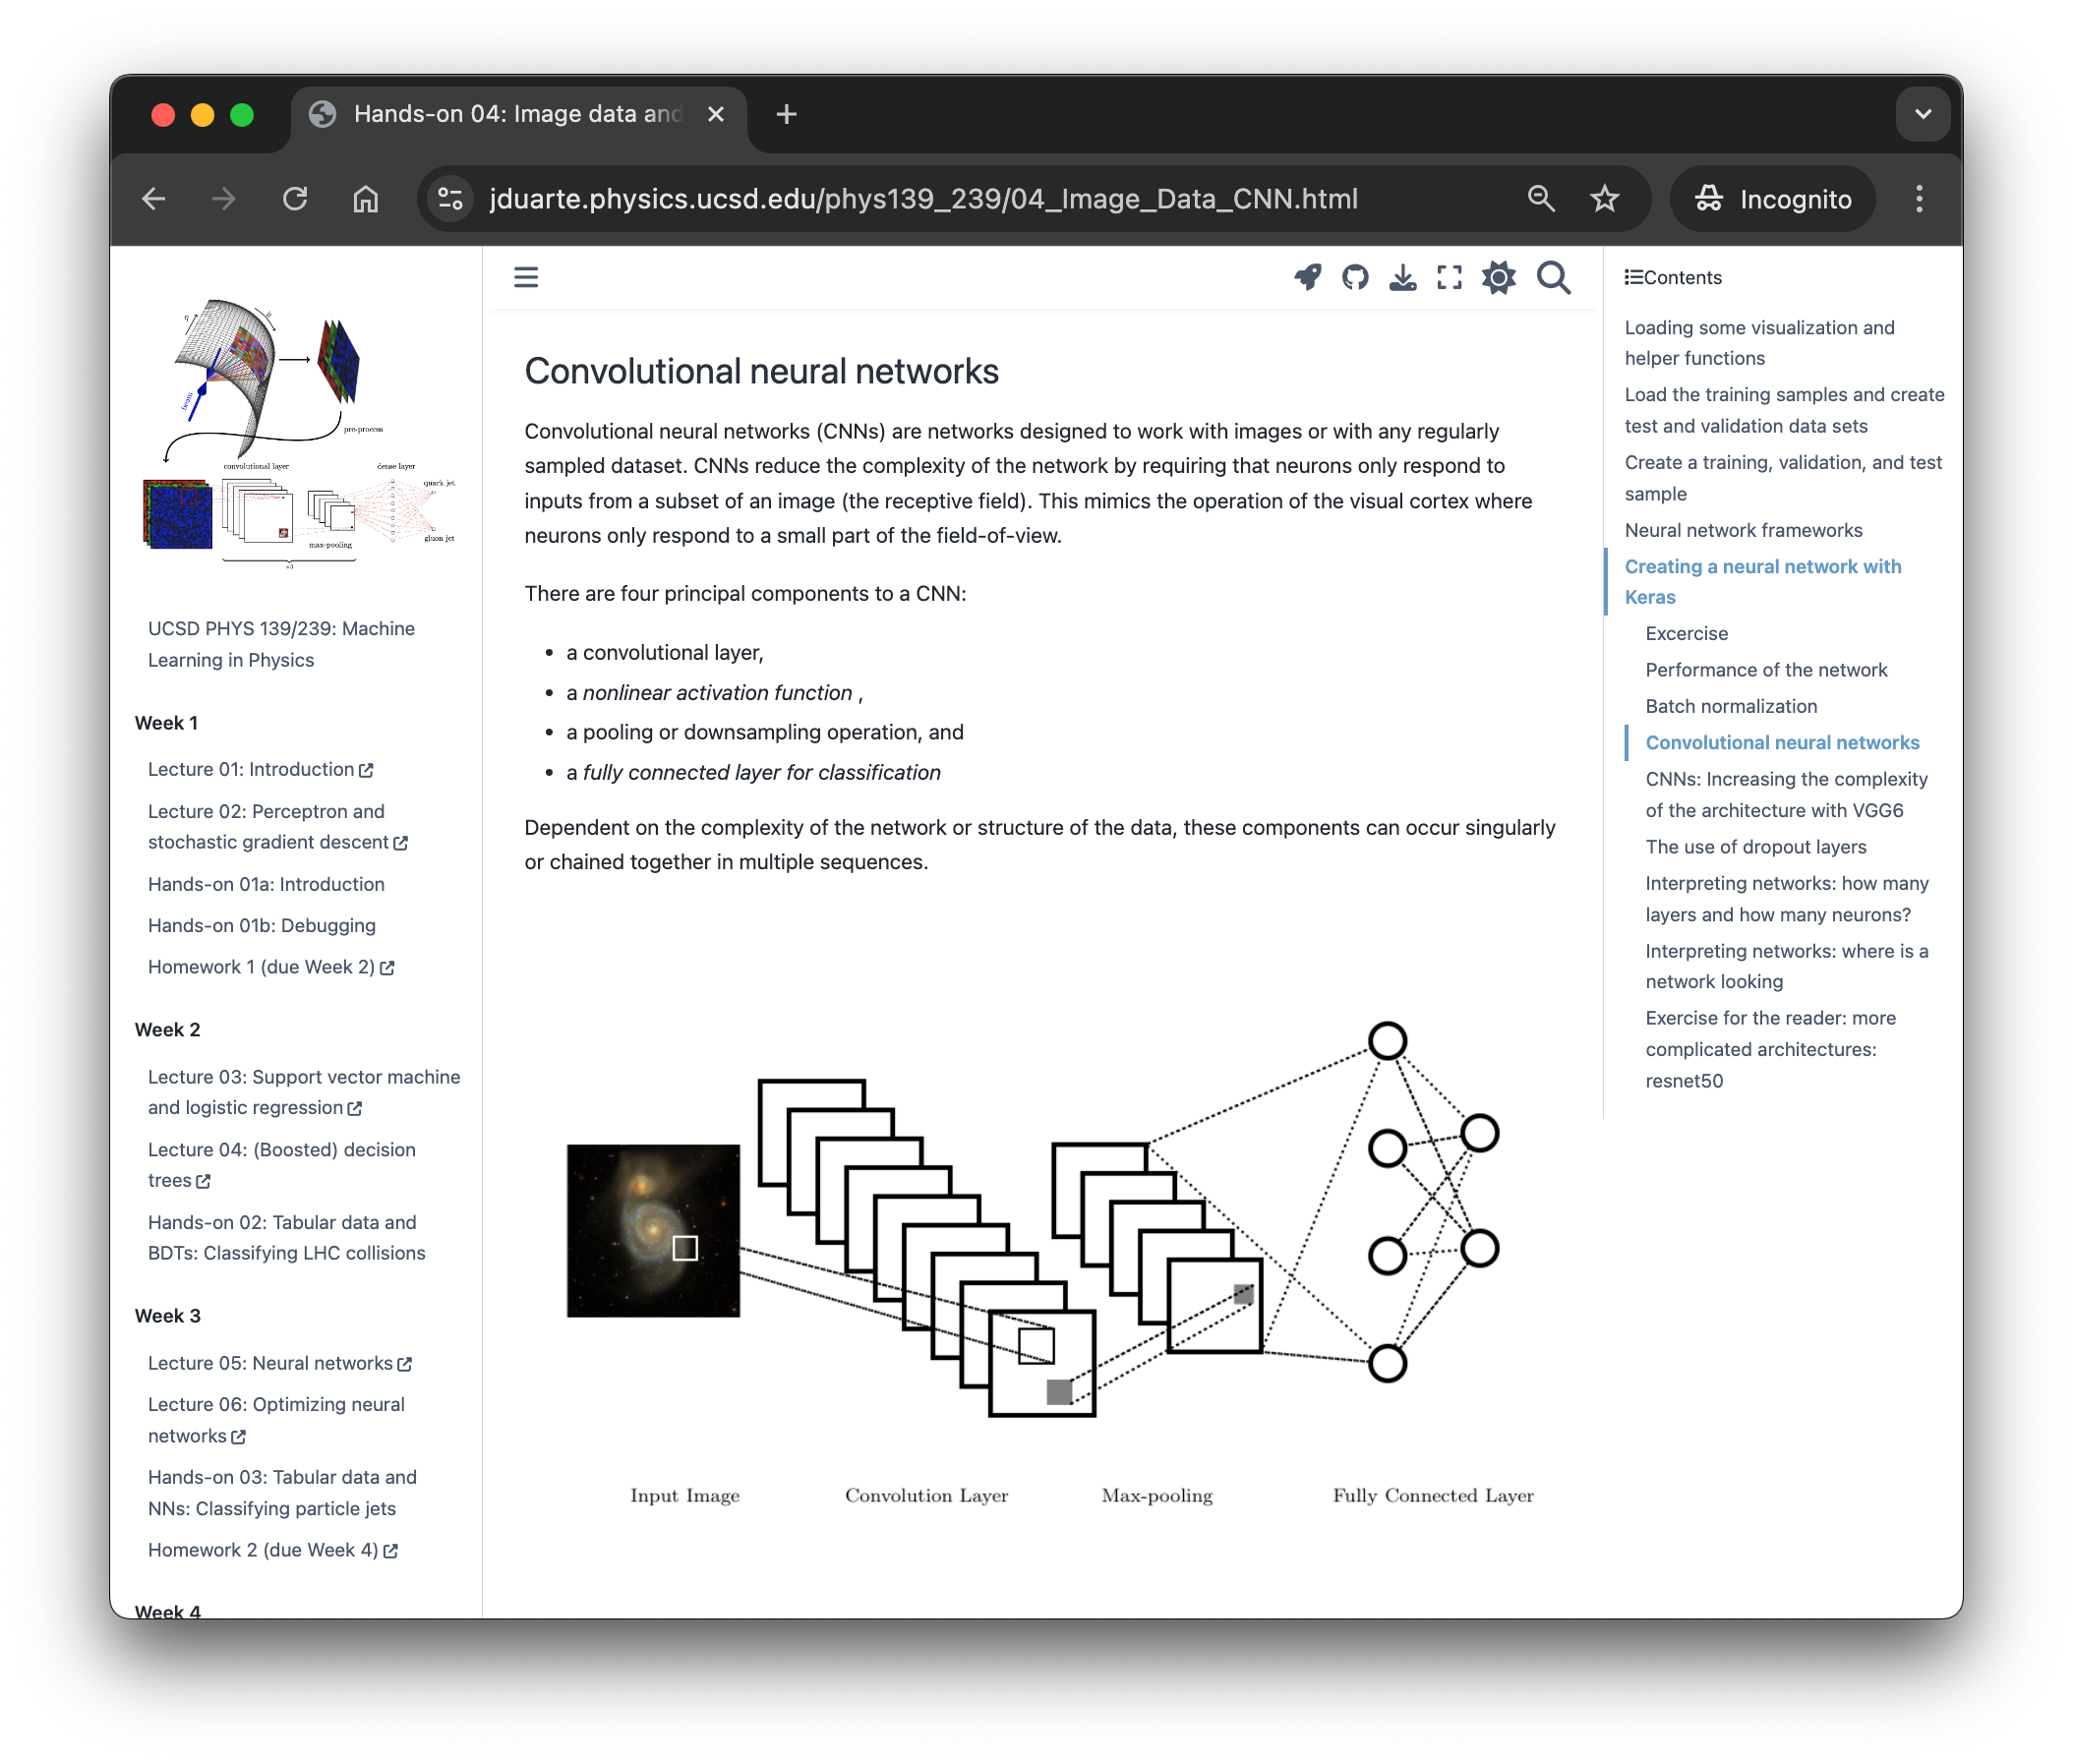
\includegraphics[width=0.35\textwidth]{jupyterbook.png}
    \includegraphics[width=0.5\textwidth]{phys141_data.pdf}
    \caption[Jupyter Book format]{Demonstration of the Jupyter Book format (left).
        The code is executable and renders in the browser.
        Visualizations of data sets used in Physics 139/239: (a) high-energy collider physics data consisting of simulated particle jets from the CMS experiment for identifying Higgs bosons, (b) astrophysical time-series data consisting of gravitational wave transient events maintained by the LIGO/Virgo/KAGRA collaboration, and (c) neutrino physics data containing simulated neutrinos interacting in a liquid argon time projection chamber (right).
        \label{fig:teaching}}
\end{figure}

I also revamped Physics 141/241: Computational Physics I: Probabilistic Models and Simulations (Winter 2022, Spring 2023) and Physics 142/242: Computational Physics II: PDE and Matrix Models (Spring 2022, Winter 2024, Winter 2025).
I helped procure modern campus computing resources through the UCSD JupyterHub Data Science and Machine Learning Platform (DSMLP).
I showed students how to use modern computing tools like Jupyter, Git, Docker, Numpy/Numba, and Kubernetes for exploratory programming, writing accelerated vectorized code, collaboration and version control, creating reproducible environments, and orchestrating jobs over large clusters.
The students gave positive feedback on gaining this experience, finding the skills transferable to computational research and job opportunities.
I also co-taught a new graduate course developed with Prof. R. Sekhar Chivukula, Physics 239: Computational Methods in Collider Physics (Spring 2023), covering beyond the SM physics, Monte Carlo event generators, detector simulation, and ML methods for data analysis.
The goal of the course is to give graduate students an ``end-to-end'' view of the process from theoretical prediction to experimental constraints.

During this review period, I taught Physics 105A: Mathematical and Computational Physics I for the first time in Winter 2025, covering Fourier series and integrals, special functions, initial and boundary value problems, and Green's functions with applications to the heat, Laplace, and wave equations.
My main goal was for students to appreciate how applying ideas from linear algebra (i.e., eigenvalues and eigenvectors) to differential equations can give us powerful tools to solve them and understand their properties.
Often, I would pose an in-class problem and ask students to solve it in small groups using the methods we had just learned, and then we would review the solution together.
I was also interested in giving students experience using computational tools, like Mathematica and open-source alternatives, to solve problems that are difficult to solve analytically, visualize the solutions, and build their intuition about the underlying physics.
The course structure consisted of three weekly lectures and two weekly computer lab sessions, with nine homework assignments, two in-class midterms, and a final exam.

I also taught Physics 2C: Fluids, Waves, Thermodynamics, and Optics to 300+ students in Spring 2026.
I adopted a ``flipped classroom'' format with readings and conceptual homework assignments due prior to each lecture.
During the lecture, I briefly reviewed the material from the readings and the homework using an iPad to write notes over prepared material, focusing on conceptually challenging issues.
I used in-class demonstrations of beat frequencies, engines, diffraction gratings, and lenses as well as a student response system (iClicker polls) to promote active learning, engage the students, and better understand the difficulties that they were having with the material.

Overall, I received good ratings in the student evaluations of teaching (SETs).
For Physics 142/242 (Winter 2025), Physics 139/239 (Fall 2025), and Physics 105A (Winter 2026), students gave scores of 4.85/5.00, 4.45/5.00, and 4.57/5.00 for student learning, 4.72/5.00, 4.36/5.00, and 4.49/5.00 for course structure, and 4.87/5.00, 4.63/5.00 and 4.61/5.00 for class environment, respectively.
For Physics 105A (Winter 2026), students wrote
\begin{quotation}
    \itshape
    The professor clearly incorporated various methods in lecture, with examples, in class problems and clear notes with steps.
    This was EXCELLENT.
    For a very hard topic, Professor Duarte did an amazing job...

    Professor Duarte has especially well-written homeworks and exams that were challenging but felt like they helped me learn or were a fair measurement of my learning.
    His lectures helped me understand course content and he was always very good about answering student questions and always took student questions seriously.
    He comes across as very knowledgable and intelligent but also incredibly humble and I especially appreciate the environment of his class...

    Professor Duarte was great! Although I mostly attended his lecture through zoom, whenever I did attend in person he would offer to stay behind and answer any questions regarding the material or homework.
    Very nice and welcoming person as well so there was never any ``fear" to come up and ask...

    Professor Duarte was very helpful when it came to helping me understand the material. What really helped was how he allowed us to use Mathematica to visualize the problems we were solving. Overall, his course provided great insight into the topics, and I really enjoyed it.
    Professor Duarte's lectures were always very well written and thought out, I left every class with a good understanding of how to solve the problems he expected us to solve.
    And the homeworks also really helped solidify the concepts that we learned...
\end{quotation}
For Physics 139/239 (Fall 2025) students wrote
\begin{quotation}
    \itshape
    The homework was a good reflection of the class material and helped me put the concepts from class into action.
    The hands-on exercises were also a good lead into the homework assignments and were a good reference for how to write the code...

    The lectures of this class are incredibly well constructed.
    They cover from the very basics all the way to some very complicated material in depth and thoroughly.
    All of the homework were incredibly relevant to the material in class, and I felt that were never anything lacking...

    The homework only ever enhanced my understanding and appreciation for the material and never took away from it, complicated it, or forced me to learn copious amounts of material on my own.
    The hands-on were engaging and provided nice places to go if I was stuck writing certain parts of my code, as I could always cross-reference with these materials. I also liked the incorporation of the final project.
    It was really interesting trying to tackle and recreate the contents of a paper in machine learning.
    I think the passion that this instructor has for this field and the examples and experience he can bring to the table make lectures really engaging. Finally, although I never went to in-depth there were a lot of supplemental reading and materials provided for this course.
    In the future if I was doing machine learning topics again, I would definitely not hesitate to return to these lectures and the materials recommended in this course...

    This was one of my favorite classes I have taken at UCSD. More than anything this class has really expanded my knowledge of what is possible with computer science, coding, and physics. I have always loved coding and solving the challenges associated with coding a program.
    But, I also loved Physics and Math and this course showed me an avenue that I could attempt to apply fuse all three of these passions or at least apply ML to these passions.
    Through this course I have gained an extreme passion for machine learning that I hope I can find a way to apply and work on in future, which is probably the highest praise I could give for any class...
\end{quotation}

% I have been internationally recognized as a teacher-scholar for my contributions to particle physics and machine learning pedagogy.
I recently co-wrote the review of ``Machine Learning'' for the Particle Data Group's 2026 Review of Particle Physics to appear in Int. J. Mod. Phys. A~[\myextcite{Duarte:2025qbk}].
These reviews are widely seen as the definitive reference material for our field, with each biannual edition typically receiving nearly 10,000 citations.
I also co-wrote the section on applications in high energy physics in an invited review for \emph{Nature Reviews Electrical Engineering} entitled ``Opportunities and challenges of graph neural networks in electrical engineering''~[\myextcite{Chien:2024gnn}].
I received a 2023 Cottrell Scholar Award from the Research Corporation for Science Advancement for my project to augment computational physics course offerings at UC San Diego entitled ``Building a Better Foundation: Teaching Physicists and Machines How to Learn from Data.''
I have co-written two textbook chapters aimed at graduate students, entitled ``Graph Neural Networks for Particle Tracking and Reconstruction'' in \emph{Artificial Intelligence for High Energy Physics}~[\myextcite{Duarte:2020ngm}] and another entitled ``Machine Learning for Analysis and Instrumentation in High Energy Physics'' in \emph{Instrumentation and Techniques in High Energy Physics}~[\myextcite{Duarte:2024xkc}].

\vspace{-1ex}
\subsection*{Service}

I served as one of the Physics Department faculty representatives for the Mentoring Project in the Division of Graduate Education and Postdoctoral Affairs (GEPA) since 2023.
As part of this initiative, I contributed to the creation of a departmental mentoring compact designed to support clear communication, shared expectations, and ongoing dialogue between mentors and mentees.
The compact is available as a resource for all members of the Physics community at\\\href{https://physics.ucsd.edu/community/mentorship}{https://physics.ucsd.edu/community/mentorship}.
We also held several community events to promote the use of the compact and to foster a culture of mentorship in the department.

During the 2025--2026 academic year, I served on the Physics Department Graduate Admissions Committee, Undergraduate Committee on Education Policy (UG-CEP), and Colloquium \& Events Committee.
% Beginning in 2022, I served as the Physics Department representative to the Equity in Graduate Education (EGE) Consortium, formerly known as the California Consortium for Inclusive Doctoral Education (C-CIDE).
As part of the Graduate Admissions Committee, I reviewed all applications for experimental astrophysics and HEP candidates using a holistic rubric I developed in collaboration with theoretical physics colleagues, following recommendations from the Equity in Graduate Education (EGE) Consortium.
In the UG-CEP, our main task has been contributing to the relevant portions of the Self-Study as part of the Division of Undergraduate Education (DUE) and GEPA Program Review of the Physics Department in 2027.
In particlar, we have been coordinating the development of a template for learning outcomes to be completed by instructors of every core course, and I am leading the writing of the learning outocomes for the computational course offerings in the Physics Department.
Finally in the Colloquium \& Events Committee, I focused on recruiting Professor Lawrence Lee (University of Tenessee, Knoxville) to discuss his work on current and future colliders.
Due to budget constraints, I sought to offset costs, by applying to and being awarded a Cottrell Lectureship, which provided \$1500 to our chosen speaker to give two colloquiua at UCSD and SDSU.

I am also a member of the School of Physical Sciences Task Force on Data Science in the Physical Sciences.
Specifically, I am chairing the subgroup on Computing and Data Infrastructure, which is responsible for assessing current computational infrastructure, identifying gaps in access or usability, and ensuring that students and instructors have access to the necessary software, hardware, and datasets to support hands-on, high-impact learning.
I have also volunteered to serve on the Ad-Hoc Committee for the Five-Year Review of Warren College Provost Marisa Abrajano.
Finally, as a member of the Executive Board of the UC San Diego Faculty Association (SDFA), I advocate for faculty interests and to advance shared governance.

I have served as a peer reviewer for \emph{J. High Energy Phys.}, \emph{Phys. Lett. B}, \emph{Phys. Rev. D}, \emph{Phys. Rev. Research}, \emph{Eur. Phys. J. C}, \emph{Comput. Softw. Big Sci.}, and \emph{Nucl. Instrum. Methods Phys. Res. A}, and \emph{Applied Optics}, and as a Guest Associate Editor for \emph{Front. Big Data} and \emph{Front. AI}.
I have also reviewed for the NeurIPS, ICML, and ICLR Conferences.
I have served as an external reviewer of grant applications for the NSF and DOE.
I am a member of the Scientific Organizing Committee for the annual Fast Machine Learning for Science Conference since 2020, and I am the lead local organizer for the 2026 conference to be held at UCSD in August 2026.
I was also a member of the Scientific Program Committee (Track 2: Data Analysis - Algorithms and Tools) for the 22nd International Workshop on Advanced Computing and Analysis Techniques in Physics Research (ACAT) in 2024.
I am one of the Energy Frontier Track Convener for APS Division of Particles and Fields (DPF) Meeting in 2026.

\vspace{-1ex}
\subsection*{Equity, Diversity, and Inclusion}

As a faculty member, I have led Equity, Diversity, and Inclusion (EDI) initiatives, especially promoting equitable graduate admissions.
I was recognized for these contributions by a UCSD Inclusive Excellence Award in 2023.
As key personnel of the NSF HDR A3D3 Institute, I co-chair the Equity and Career Committee.
One of my main contributions in this role was the conception and execution of the A3D3 Postbaccalaureate Research Fellowship.
This one-year fellowship is intended to increase research opportunities for URM groups in STEM.
In particular, the program is intended as a bridge to help students with a lack of access to research opportunities gain experience while being supported with mentoring and professional development activities (like technical writing seminars), in order to be more competitive for graduate study or industry positions.
Over the five years (2022--2027), nineteen postbaccalaureate fellows have been recruited to conduct research at institutions across the country including UCSD.
I was also a Co-PI on an NSF award to expand this program to candidates from the University of Illinois at Chicago entitled ``PREP: Advancing Research and Education in AI/ML for Science (AREAS).''

I am the lead PI on a Cottrell Scholars Collaborative titled ``Hidden Figures in Physics and Astronomy'' (\$25,000, 2023--2026) funded by the Research Corporation for Science Advancement.
The aim of this project is to create a database of URM scientists in physics and astronomy, and to develop a series of educational modules for college students to learn about the contributions of URM scientists to these fields.
A preliminary version of the database is available at\\\href{https://hiddenfigs.github.io}{hiddenfigs.github.io}.

I have also mentored students ranging from high school to graduate school participating in the SDSC MAP, UCSD EXPAND, UCSD ENLACE, UCSD STEMULATE, Cal-Bridge, CERN REU, IRIS-HEP fellowship, APS National Mentorship, and US CMS Mentorship programs.
Many of these programs specifically aim to provide opportunities for URM students in STEM.
I was a faculty co-chair of APS Conference for Undergraduate Women and Gender Minorities in Physics (CU*iP), which took place at UCSD in January 2025 and hosted more than 300 attendees from the region.
Finally, I contribute to department-level outreach activities, for example, as an exhibitor for the Physics Department and my lab at the \href{https://www.barriologansae.com/}{Barrio Logan Science \& Art Expo}.

\vspace{0.1in}
\includegraphics{signature.pdf}\\
\indent\indent Javier M. Duarte\\
\indent\indent \today

\end{document}
